\subsection{Từ LSTM đến Cơ chế Chú ý (Attention)}
Mặc dù LSTM đã giải quyết tốt vấn đề tiêu biến đạo hàm, nó vẫn gặp khó khăn khi xử lý các chuỗi cực dài. Cơ chế Chú ý (Attention Mechanism) cho phép mô hình tập trung vào những phần quan trọng nhất của chuỗi đầu vào tại mỗi bước dự báo, thay vì nén toàn bộ thông tin vào một vector trạng thái duy nhất.

\subsection{Dự báo chuỗi thời gian (Time Series Forecasting)}
Khác với phân loại văn bản, dự báo chuỗi thời gian yêu cầu mô hình nắm bắt được tính mùa vụ (seasonality), xu hướng (trend) và các biến động phi tuyến tính từ dữ liệu số.

\subsection{Thực nghiệm chuyên sâu trên 5 Datasets \& 5 Models}

\subsubsection{Dataset 1: Beijing Air Quality (LSTM + Multi-variate)}
\textbf{Kiến trúc:} LSTM đa biến.
\textbf{Mục tiêu:} Dự báo nồng độ bụi mịn PM2.5 dựa trên nhiều yếu tố khí tượng như nhiệt độ, độ ẩm, gió.
\paragraph{Thực nghiệm với Beijing Air Quality} \hfill \\
Đây là bài toán dự báo đa biến (Multivariate Time Series Forecasting). Mục tiêu là dự báo nồng độ bụi mịn PM2.5 dựa trên các yếu tố lịch sử và khí tượng như nhiệt độ, áp suất, tốc độ gió.

\paragraph{Mô hình Multivariate LSTM} \hfill \\
Mô hình sử dụng cơ chế cửa sổ trượt (sliding window) với độ dài 24 giờ (\textbf{LOOK\_BACK = 24}) để dự báo giá trị cho giờ tiếp theo. Tổng số tham số là \textbf{121,665}.

\paragraph{Kết quả thực nghiệm} \hfill \\
Mô hình đạt độ chính xác cực cao với \textbf{R² score là 0.9457}. Chỉ số \textbf{Test RMSE là 21.1601 µg/m³}.

\begin{figure}[H]
    \centering
    \begin{minipage}{0.48\textwidth}
        \centering
        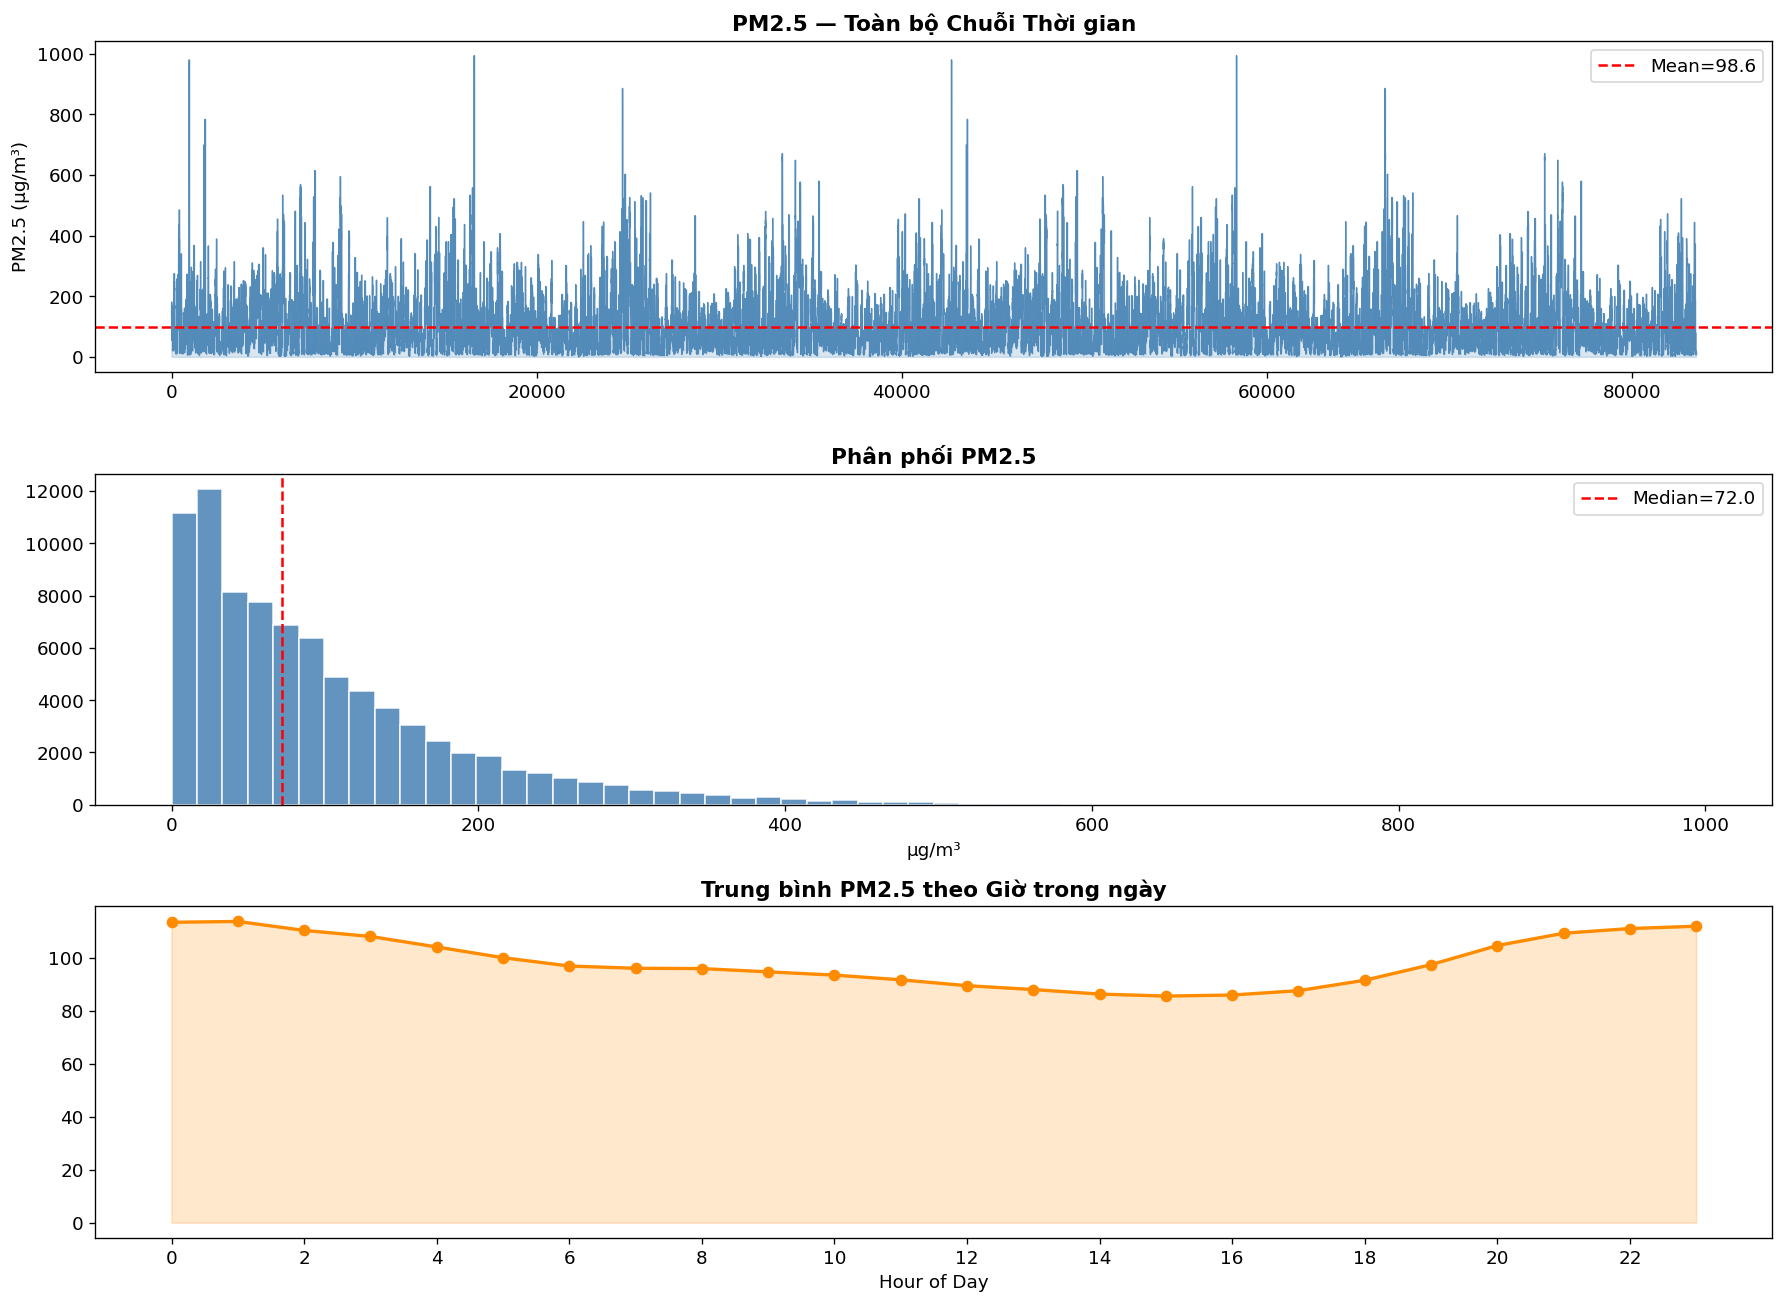
\includegraphics[width=\linewidth]{Chương_4/results/beijing_air_quality/01_time_series_eda.png}
        \caption{Biến thiên nồng độ PM2.5 theo thời gian}
        \label{fig:air_eda}
    \end{minipage}
    \hfill
    \begin{minipage}{0.48\textwidth}
        \centering
        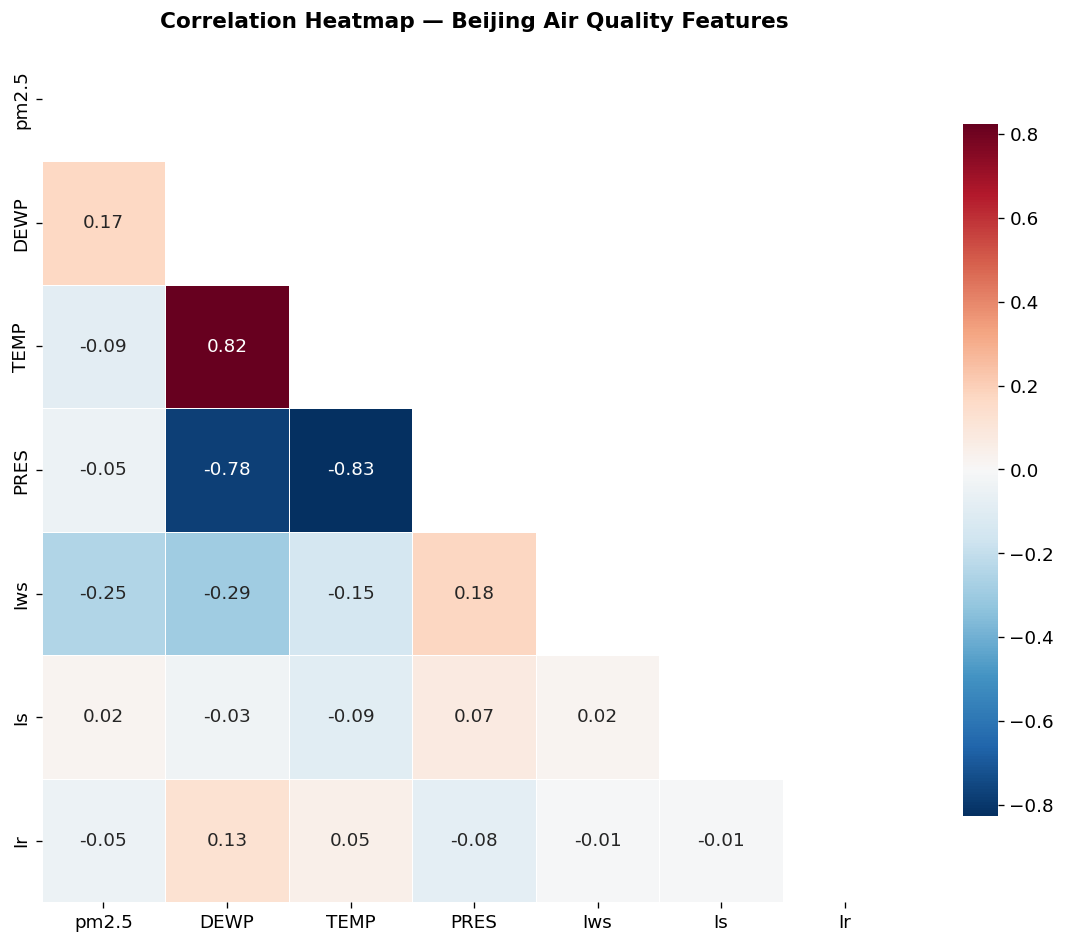
\includegraphics[width=\linewidth]{Chương_4/results/beijing_air_quality/02_correlation_heatmap.png}
        \caption{Tương quan giữa các yếu tố khí tượng}
        \label{fig:air_corr}
    \end{minipage}
\end{figure}

\begin{figure}[H]
    \centering
    \begin{minipage}{0.31\textwidth}
        \centering
        
\includegraphics[width=\linewidth]{Chương_4/results/beijing_air_quality/03_training_history.png}
        \caption{Lịch sử huấn luyện}
        \label{fig:air_history}
    \end{minipage}
    \hfill
    \begin{minipage}{0.31\textwidth}
        \centering
        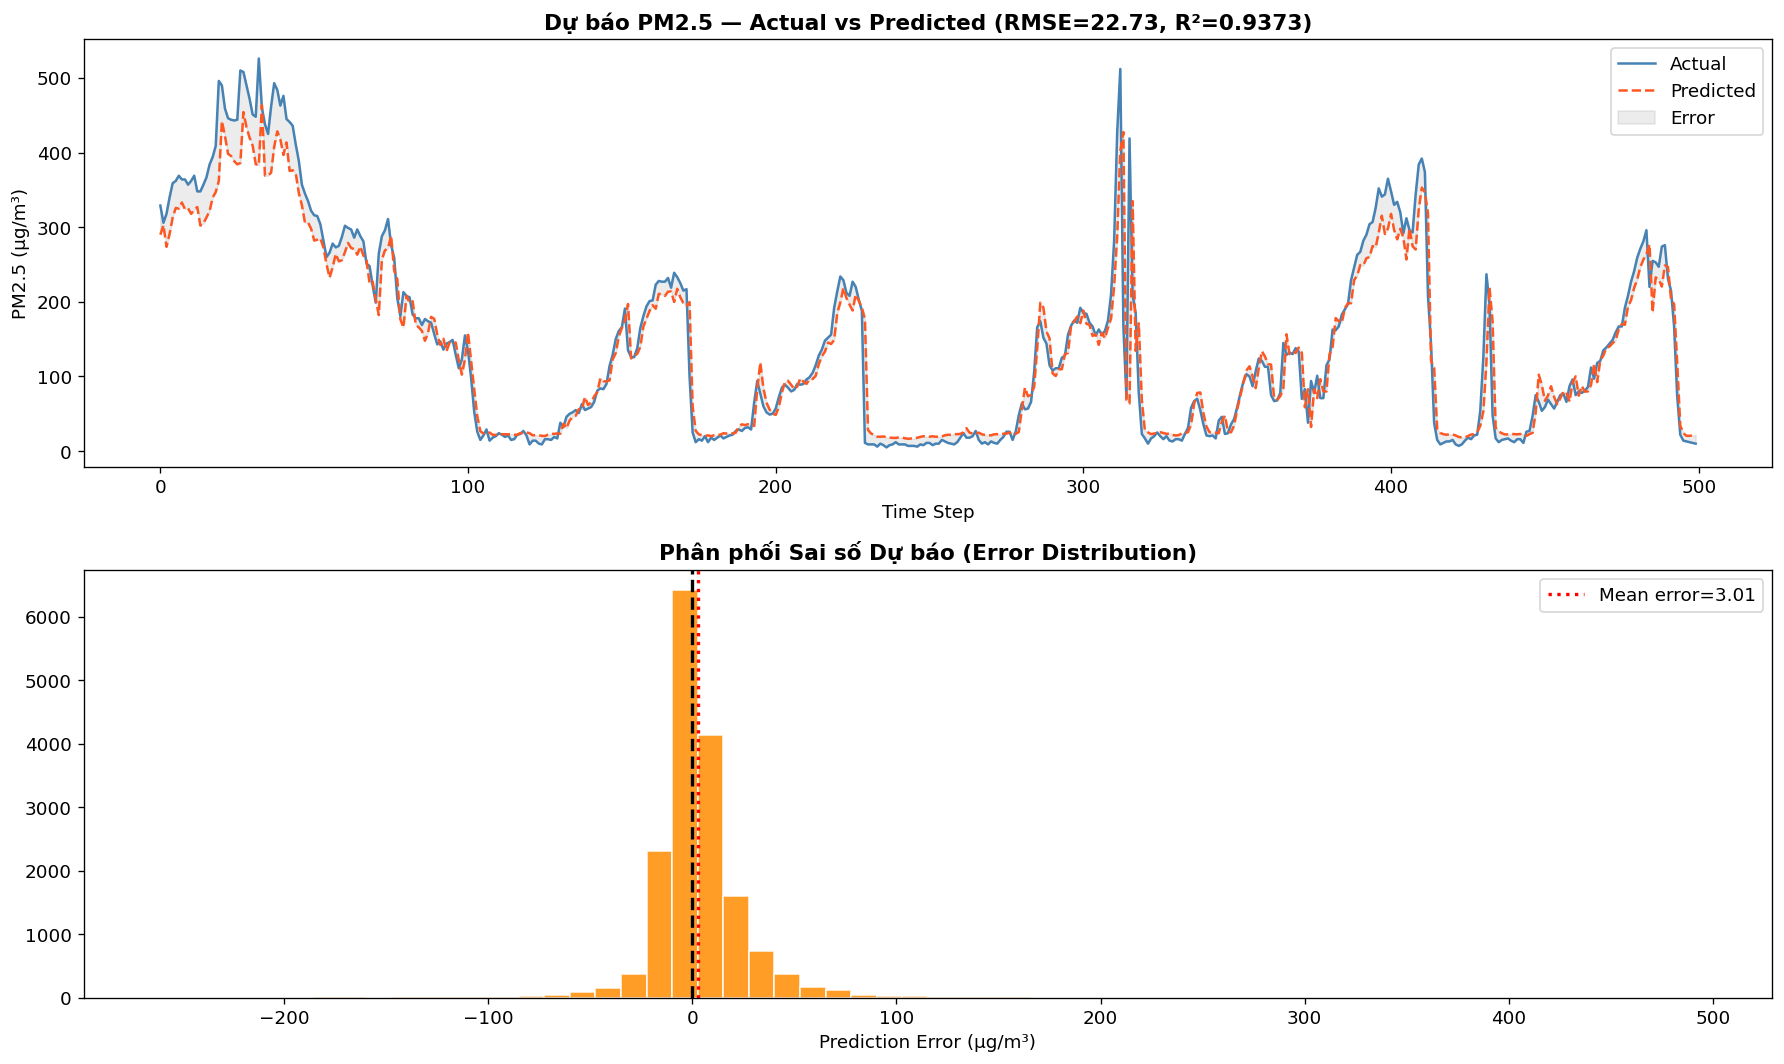
\includegraphics[width=\linewidth]{Chương_4/results/beijing_air_quality/04_forecast_vs_actual.png}
        \caption{Dự báo vs Thực tế}
        \label{fig:air_forecast}
    \end{minipage}
    \hfill
    \begin{minipage}{0.31\textwidth}
        \centering
        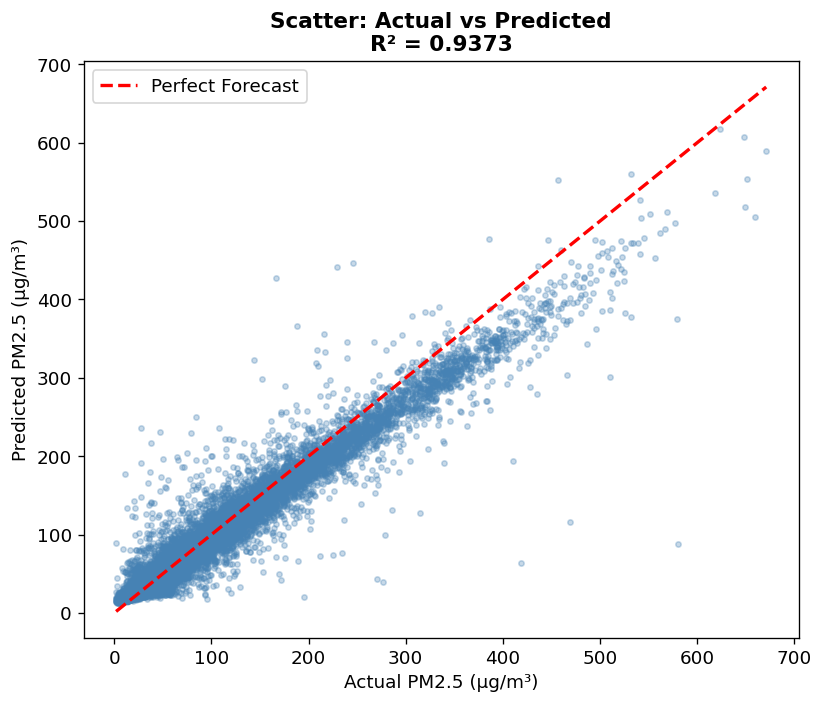
\includegraphics[width=\linewidth]{Chương_4/results/beijing_air_quality/05_scatter_actual_vs_pred.png}
        \caption{Actual vs Predicted}
        \label{fig:air_scatter}
    \end{minipage}
\end{figure}


\paragraph{Phụ lục: Quy trình thực nghiệm chi tiết} \hfill \\
Dưới đây là các bước triển khai chi tiết trên môi trường Jupyter Notebook:

\begin{figure}[H]
    \centering
    
\includegraphics[width=0.9\linewidth]{Chương_4/docs/ch4/1.png}
    \caption{Tải dữ liệu: Đọc file CSV chứa các chỉ số chất lượng không khí tại Bắc Kinh từ 2010-2014.}
\end{figure}

\begin{figure}[H]
    \centering
    
\includegraphics[width=0.9\linewidth]{Chương_4/docs/ch4/2.png}
    \caption{Kiểm tra dữ liệu thiếu: Xác định nồng độ PM2.5 bị thiếu tại một số thời điểm (NaN).}
\end{figure}

\begin{figure}[H]
    \centering
    
\includegraphics[width=0.9\linewidth]{Chương_4/docs/ch4/3.png}
    \caption{Xử lý giá trị thiếu: Sử dụng phương pháp nội suy tuyến tính (Interpolation) để lấp đầy các khoảng trống dữ liệu.}
\end{figure}

\begin{figure}[H]
    \centering
    
\includegraphics[width=0.9\linewidth]{Chương_4/docs/ch4/4.png}
    \caption{EDA chuỗi thời gian: Trực quan hóa biến động PM2.5 qua các năm để thấy rõ tính mùa vụ và xu hướng.}
\end{figure}

\begin{figure}[H]
    \centering
    
\includegraphics[width=0.9\linewidth]{Chương_4/docs/ch4/5.png}
    \caption{Trích xuất đặc trưng thời gian: Chuyển đổi các cột Year, Month, Day thành các đặc trưng số học hỗ trợ mô hình.}
\end{figure}

\begin{figure}[H]
    \centering
    
\includegraphics[width=0.9\linewidth]{Chương_4/docs/ch4/6.png}
    \caption{Chuẩn hóa dữ liệu: Sử dụng MinMaxScaler để đưa các biến khí tượng về khoảng [0, 1] nhằm tối ưu hóa hội tụ.}
\end{figure}

\begin{figure}[H]
    \centering
    
\includegraphics[width=0.9\linewidth]{Chương_4/docs/ch4/7.png}
    \caption{Chuyển đổi sang học có giám sát: Tạo cấu trúc cửa sổ trượt (sliding window) với `LOOK\_BACK = 24` giờ.}
\end{figure}

\begin{figure}[H]
    \centering
    
\includegraphics[width=0.9\linewidth]{Chương_4/docs/ch4/8.png}
    \caption{Phân tách dữ liệu: Chia tập Train/Test theo trình tự thời gian để đảm bảo tính thực tế của dự báo.}
\end{figure}

\begin{figure}[H]
    \centering
    
\includegraphics[width=0.9\linewidth]{Chương_4/docs/ch4/9.png}
    \caption{Kiến trúc Multivariate LSTM: Định nghĩa mô hình với các lớp LSTM và Dense để xử lý dữ liệu đa biến.}
\end{figure}

\begin{figure}[H]
    \centering
    
\includegraphics[width=0.9\linewidth]{Chương_4/docs/ch4/10.png}
    \caption{Nhật ký huấn luyện: Theo dõi quá trình giảm hàm mất mát (Loss) qua từng Epoch trên cả hai tập dữ liệu.}
\end{figure}

\begin{figure}[H]
    \centering
    
\includegraphics[width=0.9\linewidth]{Chương_4/docs/ch4/11.png}
    \caption{Lịch sử hội tụ: Đồ thị MSE và MAE khẳng định mô hình học ổn định và hội tụ nhanh chóng.}
\end{figure}

\begin{figure}[H]
    \centering
    
\includegraphics[width=0.9\linewidth]{Chương_4/docs/ch4/12.png}
    \caption{Mã nguồn đánh giá: Triển khai các hàm vẽ biểu đồ so sánh Dự báo vs Thực tế và phân tích sai số.}
\end{figure}

\begin{figure}[H]
    \centering
    
\includegraphics[width=0.9\linewidth]{Chương_4/docs/ch4/13.png}
    \caption{Kết quả dự báo chi tiết: Đồ thị đường bám sát giá trị thực tế và biểu đồ phân phối sai số tập trung quanh mức 0.}
\end{figure}

\begin{figure}[H]
    \centering
    
\includegraphics[width=0.9\linewidth]{Chương_4/docs/ch4/14.png}
    \caption{Biểu đồ phân tán (Scatter Plot): Sự tương quan chặt chẽ giữa giá trị thực tế và dự đoán ($R^2 = 0.9457$).}
\end{figure}


\subsubsection{Dataset 2: Google Stock Price (Conv1D + LSTM)}
\textbf{Kiến trúc:} Kết hợp Convolutional 1D và LSTM.
\textbf{Mục tiêu:} Sử dụng Conv1D để trích xuất đặc trưng cục bộ và LSTM để học xu hướng dài hạn của giá cổ phiếu.
\paragraph{Thực nghiệm với Google Stock Price} \hfill \\
Dự báo giá cổ phiếu là một trong những bài toán khó nhất do tính nhiễu và sự biến động mạnh của thị trường tài chính.

\paragraph{Mô hình Conv1D + LSTM} \hfill \\
Chúng ta kết hợp lớp \textbf{Conv1D} để lọc nhiễu và trích xuất các đặc trưng cục bộ (pattern) ngắn hạn, sau đó đưa vào lớp \textbf{LSTM} để học các xu hướng dài hạn. Cửa sổ quan sát được thiết lập là 60 ngày (\textbf{LOOK\_BACK = 60}).

\paragraph{Kết quả và Phân tích} \hfill \\
Mô hình đạt \textbf{R² score là 0.9745} và \textbf{Test RMSE là 22.37 USD}. Biểu đồ dự báo cho thấy mô hình bắt kịp các xu hướng tăng giảm chính của mã cổ phiếu GOOGL.

\begin{figure}[H]
    \centering
    \begin{minipage}{0.48\textwidth}
        \centering
        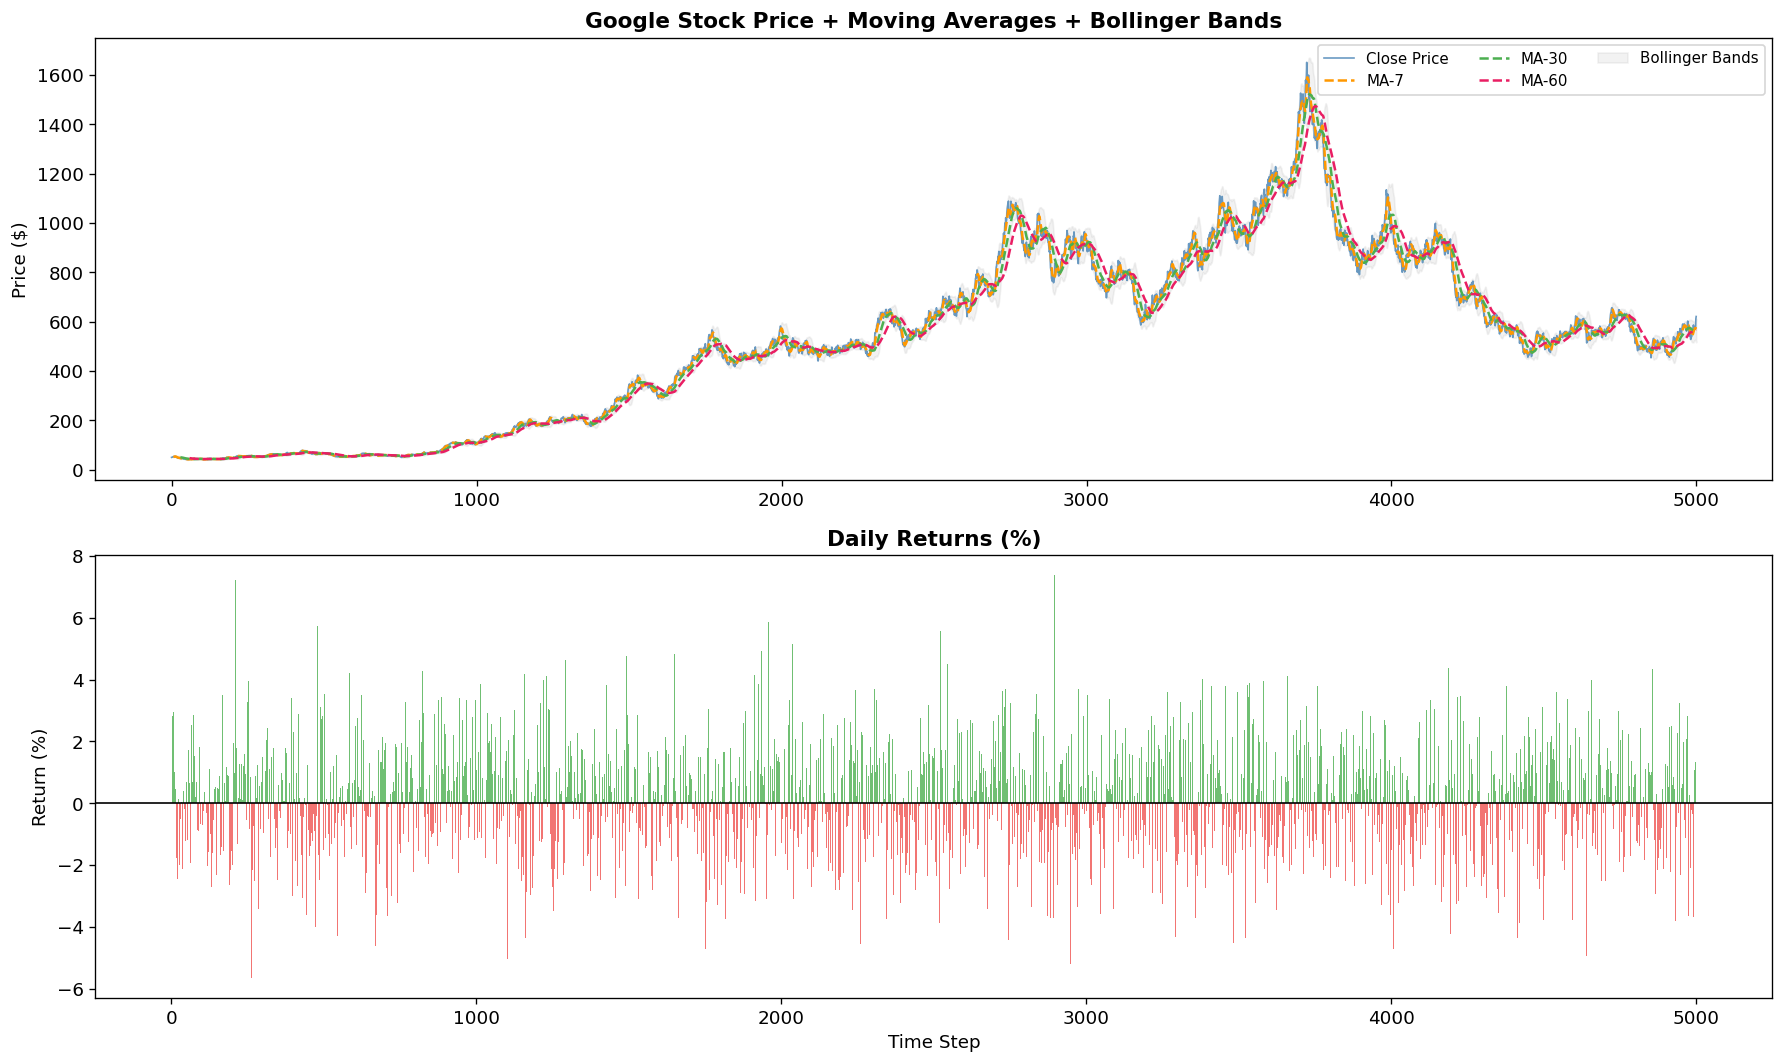
\includegraphics[width=\linewidth]{Chương_4/results/google_stock/01_stock_eda.png}
        \caption{Biến động giá cổ phiếu Google (Lịch sử)}
        \label{fig:stock_eda}
    \end{minipage}
    \hfill
    \begin{minipage}{0.48\textwidth}
        \centering
        \includegraphics[width=\linewidth]{Chương_4/results/google_stock/02_returns_volatility.png}
        \caption{Phân tích lợi nhuận và độ biến động}
        \label{fig:stock_vol}
    \end{minipage}
\end{figure}

\begin{figure}[H]
    \centering
    \includegraphics[width=0.8\linewidth]{Chương_4/results/google_stock/03_forecast_results.png}
    \caption{Kết quả dự báo giá cổ phiếu trên tập kiểm tra}
    \label{fig:stock_forecast}
\end{figure}


\paragraph{Phụ lục: Quy trình thực nghiệm chi tiết} \hfill \\
Dưới đây là các bước triển khai chi tiết trên môi trường Jupyter Notebook:

\begin{figure}[H]
    \centering
    
\includegraphics[width=0.9\linewidth]{Chương_4/docs/ch4/15.png}
    \caption{Tải dữ liệu tài chính: Đọc lịch sử giá cổ phiếu Google (GOOG) bao gồm các cột giá Open, High, Low, Close và Volume.}
\end{figure}

\begin{figure}[H]
    \centering
    
\includegraphics[width=0.9\linewidth]{Chương_4/docs/ch4/16.png}
    \caption{EDA giá cổ phiếu: Trực quan hóa sự tăng trưởng dài hạn và các giai đoạn biến động mạnh của thị trường.}
\end{figure}

\begin{figure}[H]
    \centering
    
\includegraphics[width=0.9\linewidth]{Chương_4/docs/ch4/17.png}
    \caption{Feature Engineering nâng cao: Tính toán các chỉ số bổ sung từ giá đóng cửa và khối lượng giao dịch.}
\end{figure}

\begin{figure}[H]
    \centering
    
\includegraphics[width=0.9\linewidth]{Chương_4/docs/ch4/18.png}
    \caption{Tiền xử lý chuỗi: Chuẩn hóa và tạo cửa sổ dữ liệu quan sát (`LOOK\_BACK = 60`) để dự báo xu hướng tiếp theo.}
\end{figure}

\begin{figure}[H]
    \centering
    
\includegraphics[width=0.9\linewidth]{Chương_4/docs/ch4/19.png}
    \caption{Kiến trúc Conv1D-LSTM: Kết hợp lớp Convolution 1D để lọc nhiễu và LSTM để ghi nhớ các đặc trưng dài hạn.}
\end{figure}

\begin{figure}[H]
    \centering
    
\includegraphics[width=0.9\linewidth]{Chương_4/docs/ch4/20.png}
    \caption{Quá trình huấn luyện: Nhật ký thực thi cho thấy sự sụt giảm nhanh chóng của MSE Loss trên cả hai tập dữ liệu.}
\end{figure}

\begin{figure}[H]
    \centering
    
\includegraphics[width=0.9\linewidth]{Chương_4/docs/ch4/22.png}
    \caption{Kết quả Training History: Đồ thị Loss hội tụ tốt sau 20 epochs, không xuất hiện hiện tượng Overfitting.}
\end{figure}

\begin{figure}[H]
    \centering
    
\includegraphics[width=0.9\linewidth]{Chương_4/docs/ch4/23.png}
    \caption{Tổng kết thực nghiệm: Bản tóm tắt trực quan bao gồm Lịch sử huấn luyện, Dự báo toàn cục và Biểu đồ tương quan Scatter Plot ($R^2 = 0.9745$).}
\end{figure}


\subsubsection{Dataset 3: Energy Consumption (LSTM + Attention)}
\textbf{Kiến trúc:} LSTM kết hợp Cơ chế Chú ý (Attention).
\textbf{Mục tiêu:} Dự báo phụ tải điện năng, giải quyết tính mùa vụ mạnh và trích xuất trọng số giải thích (Explainable AI).
\paragraph{Thực nghiệm: Dự báo Tiêu thụ Năng lượng (Energy Consumption) với kiến trúc LSTM và Cơ chế Chú ý (Attention Mechanism)} \hfill\mbox{}

Bài toán dự báo phụ tải điện năng (Energy Load Forecasting) đòi hỏi hệ thống phải nắm bắt được tính mùa vụ mạnh mẽ của điện năng (chu kỳ sinh hoạt theo giờ, ngày, tuần). Mạng LSTM truyền thống tuy giải quyết tốt chuỗi thời gian nhưng thường bị suy giảm bộ nhớ khi chuỗi quá dài. Để khắc phục, chúng ta nâng cấp mạng LSTM bằng cách tích hợp \textbf{Cơ chế Chú ý (Attention Mechanism)}. Cơ chế này cho phép mô hình tự động phân bổ trọng số (attention weights), từ đó tập trung vào những mốc thời gian quá khứ có sức ảnh hưởng lớn nhất đối với giá trị tương lai.

\paragraph{Khai báo thư viện và Cấu hình ban đầu} \hfill\mbox{}

Đầu tiên, quá trình phân tích yêu cầu sử dụng các thư viện như Pandas, NumPy để tính toán, Matplotlib, Seaborn để trực quan hóa, và TensorFlow/Keras để xây dựng mô hình Deep Learning. Việc cố định seed giúp đảm bảo tính tái lập (reproducibility) cho kết quả thực nghiệm.

\begin{lstlisting}[style=pythoncode, caption={Khai báo thư viện và thiết lập môi trường}]
import pandas as pd
import numpy as np
import matplotlib.pyplot as plt
import seaborn as sns
import tensorflow as tf
from tensorflow.keras import layers, models
from sklearn.preprocessing import MinMaxScaler
from sklearn.metrics import mean_squared_error, mean_absolute_error, r2_score
import glob, os, warnings

import random

SEED = 42

np.random.seed(SEED)
random.seed(SEED)
tf.random.set_seed(SEED)
os.environ["PYTHONHASHSEED"] = str(SEED)

warnings.filterwarnings('ignore')
plt.rcParams.update({'figure.dpi': 120, 'font.size': 11,
                     'axes.titlesize': 13, 'axes.titleweight': 'bold'})

DATA_DIR   = '../data/energy_consumption'
SAVE_DIR   = '../results/energy_attention'
os.makedirs(SAVE_DIR, exist_ok=True)

LOOK_BACK  = 48    # 48 timesteps
EPOCHS     = 40
BATCH_SIZE = 64

print(f'TF: {tf.__version__}')
\end{lstlisting}

\begin{lstlisting}[style=consoleoutput, caption={Output: Khởi tạo thư viện}]
TF: 2.21.0
\end{lstlisting}

\paragraph{Tiền xử lý và Khám phá Dữ liệu (EDA)} \hfill\mbox{}

Quá trình đọc và xử lý dữ liệu bắt đầu bằng việc tìm kiếm tập dữ liệu lớn nhất trong thư mục, định dạng lại cột thời gian (\texttt{Datetime}) và xử lý các giá trị khuyết thiếu bằng kỹ thuật nội suy (\textit{Forward-fill} và \textit{Backward-fill}).

\begin{lstlisting}[style=pythoncode, caption={Đọc dữ liệu và xử lý giá trị khuyết thiếu}]
csv_files=glob.glob(f'{DATA_DIR}/**/*.csv',recursive=True)+glob.glob(f'{DATA_DIR}/*.csv')
print('Found:',csv_files)

# get the largest file
df=pd.read_csv(sorted(csv_files,key=os.path.getsize,reverse=True)[0])

# parse datetime
df['Datetime']=pd.to_datetime(df['Datetime'])
df=df.sort_values('Datetime').reset_index(drop=True)

# handle NaN values
df=df.ffill().bfill()

print('Shape:',df.shape)
print('Columns:',list(df.columns))
print('\nMissing values:\n',df.isna().sum())

df.head()
\end{lstlisting}

\begin{lstlisting}[style=consoleoutput, caption={Output: Dữ liệu tải lên}]
Found: ['../data/energy_consumption/NI_hourly.csv', ...]
Shape: (178262, 13)
Columns: ['Datetime', 'AEP', 'COMED', 'DAYTON', 'DEOK', 'DOM', 'DUQ', 'EKPC', 'FE', 'NI', 'PJME', 'PJMW', 'PJM_Load']

Missing values:
Datetime    0
AEP         0
COMED       0
DAYTON      0
DEOK        0
DOM         0
DUQ         0
EKPC        0
FE          0
NI          0
PJME        0
PJMW        0
PJM_Load    0
dtype: int64
             Datetime      AEP   COMED  DAYTON    DEOK     DOM     DUQ  \
0 1998-04-01 01:00:00  12379.0  9631.0  1621.0  2533.0  7190.0  1364.0   
1 1998-04-01 02:00:00  12379.0  9631.0  1621.0  2533.0  7190.0  1364.0   
2 1998-04-01 03:00:00  12379.0  9631.0  1621.0  2533.0  7190.0  1364.0   
3 1998-04-01 04:00:00  12379.0  9631.0  1621.0  2533.0  7190.0  1364.0   
4 1998-04-01 05:00:00  12379.0  9631.0  1621.0  2533.0  7190.0  1364.0   
\end{lstlisting}

Tiếp theo, ta tự động xác định biến mục tiêu (cột điện năng) và giới hạn ở $20,000$ điểm dữ liệu cuối cùng để tối ưu thời gian huấn luyện mà vẫn giữ được tính chất đặc trưng của tập dữ liệu chuỗi thời gian.

\begin{lstlisting}[style=pythoncode, caption={Lựa chọn biến mục tiêu (Target) và lấy mẫu (Sampling)}]
# Detect target (energy/MW/consumption)
energy_cols = [c for c in df.columns if any(k in c.lower()
               for k in ['mw','energy','consumption','kwh','load','demand'])]
TARGET_COL = energy_cols[0] if energy_cols else df.select_dtypes(include=np.number).columns[0]
print(f'Target column: {TARGET_COL}')

# Parse datetime if available
date_cols = [c for c in df.columns if any(k in c.lower() for k in ['date','time','datetime'])]
if date_cols:
    df[date_cols[0]] = pd.to_datetime(df[date_cols[0]], errors='coerce')
    df = df.dropna(subset=[date_cols[0]]).sort_values(date_cols[0]).reset_index(drop=True)

df = df.dropna(subset=[TARGET_COL])
data_series = df[TARGET_COL].values.astype(float)
print(f'Total time steps: {len(data_series):,}')

# Limit to last 20000 for speed
if len(data_series) > 20000:
    data_series = data_series[-20000:]
    print(f'Trimmed to last 20,000 steps')
\end{lstlisting}

\begin{lstlisting}[style=consoleoutput, caption={Output: Lựa chọn cột Target}]
Target column: PJMW
Total time steps: 178,262
Trimmed to last 20,000 steps
\end{lstlisting}

Để hiểu rõ cấu trúc của chuỗi thời gian, ta tiến hành vẽ đồ thị diễn biến của năng lượng.

\begin{lstlisting}[style=pythoncode, caption={Trực quan hóa diễn biến chuỗi thời gian}]
fig, axes = plt.subplots(3, 1, figsize=(15, 11))

# Full series
axes[0].plot(data_series, color='#2196F3', lw=0.8, alpha=0.9)
axes[0].fill_between(range(len(data_series)), data_series,
                     data_series.min(), alpha=0.15, color='#2196F3')
axes[0].set_title(f'{TARGET_COL} - Full Time Series')
axes[0].set_ylabel('Energy (MW)')

# Rolling stats
s = pd.Series(data_series)
roll_mean = s.rolling(window=168).mean()  # 7-day (168 hrs)
roll_std  = s.rolling(window=168).std()

axes[1].plot(data_series, color='#2196F3', lw=0.5, alpha=0.5, label='Raw')
axes[1].plot(roll_mean, color='#FF9800', lw=2, label='7-Day Rolling Mean')
axes[1].fill_between(range(len(data_series)),
                     (roll_mean + 2*roll_std).values,
                     (roll_mean - 2*roll_std).values,
                     alpha=0.15, color='#FF9800', label='+/- 2-sigma Band')
axes[1].set_title('Rolling Mean +/- 2-sigma (7-Day Window)')
axes[1].legend(fontsize=9)

# Zoom: 1 week
show = min(168, len(data_series))
axes[2].plot(data_series[:show], 'o-', color='#E91E63', lw=1.5, ms=3)
axes[2].fill_between(range(show), data_series[:show],
                     data_series[:show].min(), alpha=0.2, color='#E91E63')
axes[2].set_title(f'Zoom: First {show} steps (~1 week)')
axes[2].set_xlabel('Time Step')

plt.tight_layout()
plt.savefig(f'{SAVE_DIR}/01_energy_eda.png', bbox_inches='tight')
plt.show()

print(f'Mean: {data_series.mean():.2f} | Std: {data_series.std():.2f} | '
      f'Min: {data_series.min():.2f} | Max: {data_series.max():.2f}')
\end{lstlisting}

\begin{lstlisting}[style=consoleoutput, caption={Output: Thống kê cơ bản}]
Mean: 5583.61 | Std: 1001.56 | Min: 3420.00 | Max: 9342.00
\end{lstlisting}

\begin{figure}[H]
    \centering
    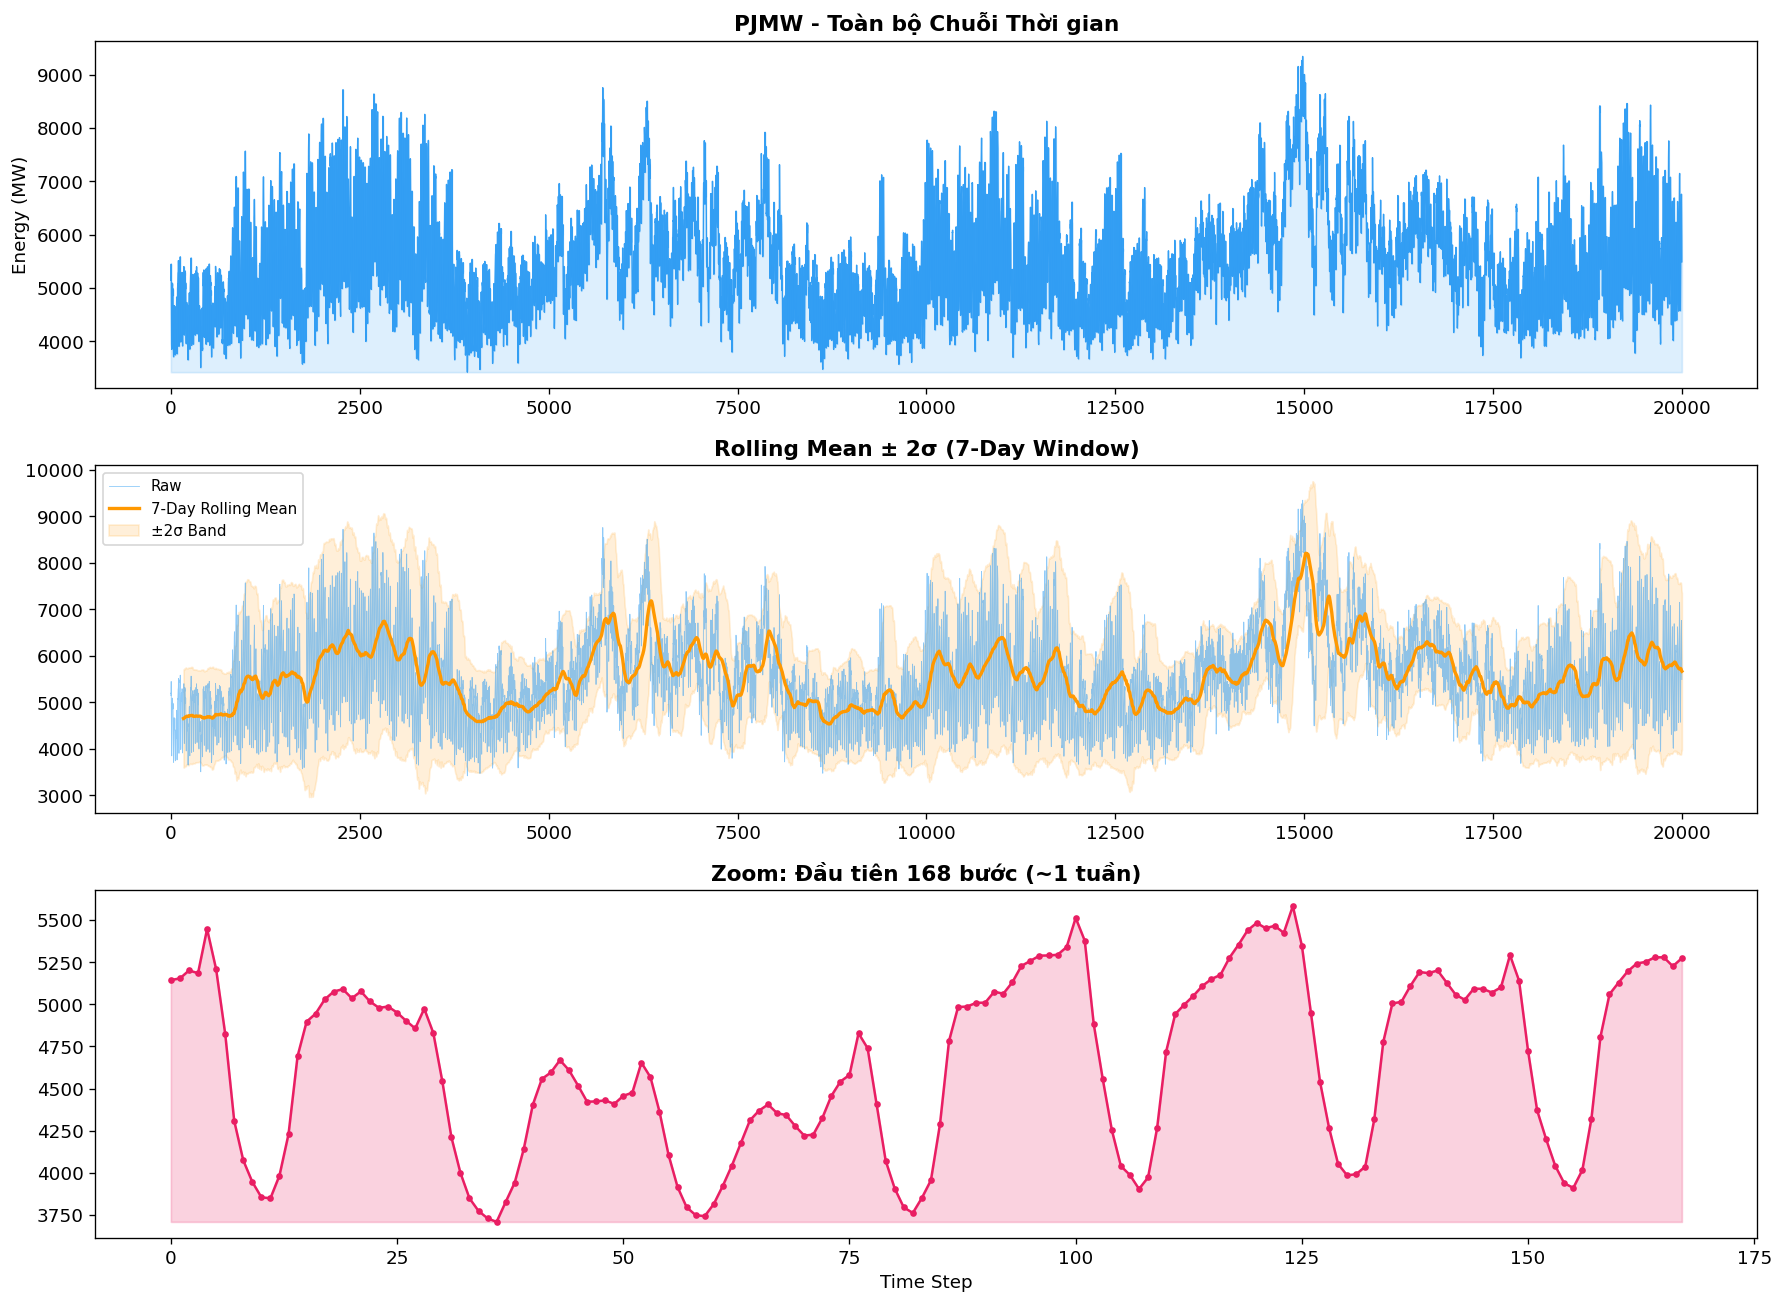
\includegraphics[width=\linewidth]{Chương_4/results/energy_attention/01_energy_eda.png}
    \caption{Chuỗi thời gian tổng thể, Rolling Mean 7 ngày và Zoom in 1 tuần}
\end{figure}

\textbf{Giải thích đồ thị:} Đồ thị dưới cùng (\textit{Zoom in 1 tuần}) thể hiện rõ ràng tính chu kỳ lặp lại theo nhịp độ sinh hoạt ngày và đêm, với các đỉnh cao vào ban ngày và đáy vào ban đêm. Đồ thị trung bình lăn (\textit{7-Day Rolling Mean}) cho thấy các xu hướng vĩ mô hơn trong tuần, với các dải $\pm 2\sigma$ chỉ ra biên độ biến động của phụ tải. Mức tiêu thụ thấp nhất là $3420$ MW và cao nhất lên tới $9342$ MW.

Để chứng minh mặt toán học của tính chu kỳ, ta phân tích phân phối dữ liệu và sử dụng hàm Tự tương quan (Autocorrelation) nhằm đo mức độ tương quan của chuỗi dữ liệu ở thời điểm $t$ so với thời điểm $t-lag$.

\begin{lstlisting}[style=pythoncode, caption={Phân phối và Tự tương quan (Autocorrelation)}]
# 1. Distribution of Energy Consumption
plt.figure(figsize=(7.5, 4.5))
mean_val = np.mean(data_series)
plt.hist(data_series, bins=60, color='#2196F3', edgecolor='white', alpha=0.85, label='Energy Distribution')
plt.axvline(mean_val, color='red', linestyle='--', lw=2, label=f'Mean = {mean_val:.2f}')
plt.title('Energy Consumption Distribution', fontsize=12, fontweight='bold', pad=12)
plt.xlabel('Energy (MW or kWh)')
plt.ylabel('Frequency')
plt.grid(True, linestyle='--', alpha=0.5)
plt.legend(frameon=True, facecolor='white', edgecolor='none')
plt.tight_layout()
plt.savefig(f'{SAVE_DIR}/02_a_energy_distribution.png', dpi=120, bbox_inches='tight')
plt.show()

# 2. Autocorrelation Analysis
plt.figure(figsize=(8.5, 4.5))
max_lag = 100
autocorr = [pd.Series(data_series).autocorr(lag=l) for l in range(1, max_lag + 1)]
plt.bar(range(1, max_lag + 1), autocorr, color='steelblue', alpha=0.8, label='Autocorrelation')
plt.axhline(0, color='black', lw=1)
plt.axhline(0.05, color='red', linestyle='--', lw=1.5, label='+/- 0.05 Confidence Interval')
plt.axhline(-0.05, color='red', linestyle='--', lw=1.5)
plt.title('Autocorrelation (lag 1-100)', fontsize=12, fontweight='bold', pad=12)
plt.xlabel('Lag')
plt.ylabel('Autocorrelation Coefficient')
plt.grid(True, linestyle='--', alpha=0.5)
plt.legend(frameon=True, facecolor='white', edgecolor='none')
plt.tight_layout()
plt.savefig(f'{SAVE_DIR}/02_b_autocorrelation.png', dpi=120, bbox_inches='tight')
plt.show()
\end{lstlisting}

\begin{figure}[H]
    \centering
    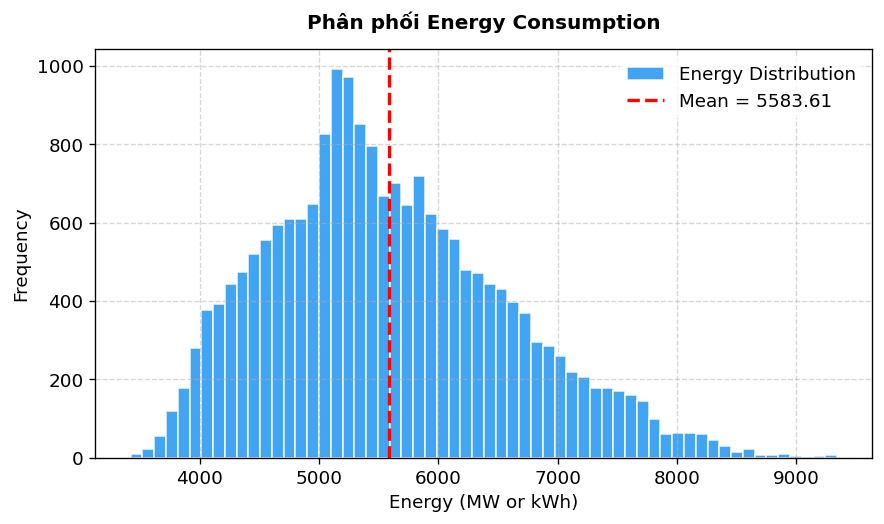
\includegraphics[width=\linewidth]{Chương_4/results/energy_attention/02_a_energy_distribution.png}
    \caption{Phân phối điện năng (Dạng hình chuông)}
\end{figure}

\textbf{Giải thích đồ thị:} Biểu đồ phân phối năng lượng cho thấy phụ tải phân bố tương đối đối xứng (dạng hình chuông) xung quanh giá trị trung bình $\approx 5583$ MW. Đặc điểm phân phối chuẩn này giúp cho mạng nơ-ron dễ dàng học và dự báo hơn so với các chuỗi dữ liệu có nhiều đuôi béo (fat-tails) hay ngoại lai cực đoan (extreme outliers) như trong thị trường tài chính.

\begin{figure}[H]
    \centering
    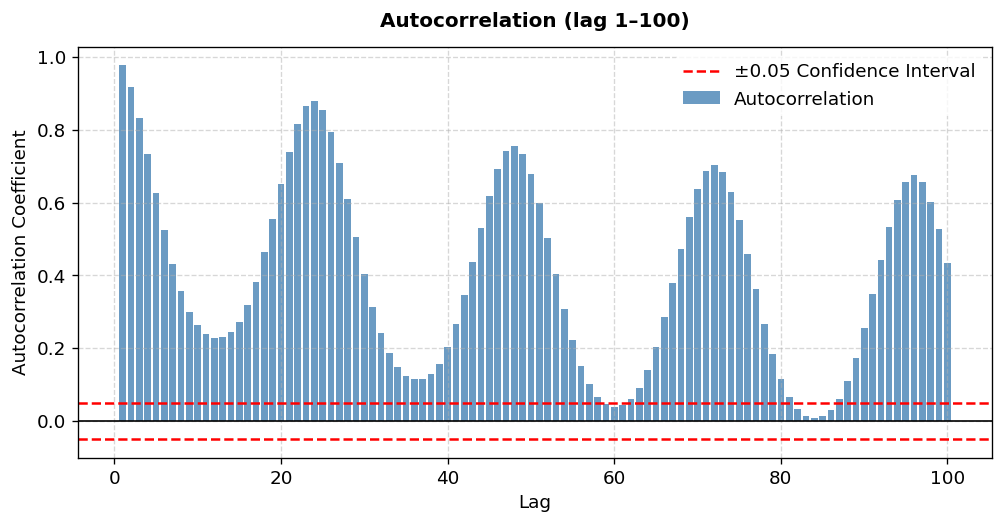
\includegraphics[width=\linewidth]{Chương_4/results/energy_attention/02_b_autocorrelation.png}
    \caption{Hệ số Tự tương quan từ lag 1 đến 100}
\end{figure}

\textbf{Giải thích đồ thị:} Biểu đồ Autocorrelation cho thấy các đỉnh sóng nhấp nhô cực kỳ đều đặn vượt qua ngưỡng tin cậy thống kê (vùng nét đứt màu đỏ). Các đỉnh sóng nhô cao nhất tương ứng với các độ trễ (lags) là bội số của 24 ($24, 48, 72 \dots$). Điều này minh chứng mạnh mẽ rằng điện năng tiêu thụ của một giờ cụ thể trong ngày hôm nay phụ thuộc tuyến tính rất lớn vào cùng giờ đó ở các ngày trước, củng cố tính chu kỳ sinh hoạt 24h vững chắc của dữ liệu.

\paragraph{Chuẩn bị Dữ liệu Huấn luyện} \hfill\mbox{}

Mạng nơ-ron hoạt động ổn định nhất khi dữ liệu được chuẩn hóa (Min-Max Scaling) về khoảng $[0, 1]$. Sau đó, ta tạo tập dữ liệu dưới dạng cửa sổ trượt (sliding window) với độ trễ \texttt{LOOK\_BACK = 48} (tương đương 48 giờ quá khứ để dự báo giờ tiếp theo) và chia tập huấn luyện/kiểm thử theo tỉ lệ 80:20.

\begin{lstlisting}[style=pythoncode, caption={Scale dữ liệu và tạo chuỗi Data Window}]
scaler = MinMaxScaler()
data_scaled = scaler.fit_transform(data_series.reshape(-1,1)).flatten()

def create_dataset(data, look_back):
    X, y = [], []
    for i in range(len(data) - look_back):
        X.append(data[i:i+look_back])
        y.append(data[i+look_back])
    return np.array(X), np.array(y)

X, y = create_dataset(data_scaled, LOOK_BACK)
X = X.reshape(X.shape[0], X.shape[1], 1)

split = int(len(X) * 0.8)
X_train, X_test = X[:split], X[split:]
y_train, y_test = y[:split], y[split:]

print(f'X: {X.shape} -> Train: {X_train.shape}, Test: {X_test.shape}')
\end{lstlisting}

\begin{lstlisting}[style=consoleoutput, caption={Output: Kích thước tập dữ liệu}]
X: (19952, 48, 1) -> Train: (15961, 48, 1), Test: (3991, 48, 1)
\end{lstlisting}

\paragraph{Xây dựng Kiến trúc Mô hình (LSTM + Attention)} \hfill\mbox{}

Thay vì sử dụng các biến thể Attention có sẵn, ta tự định nghĩa một lớp \textbf{Bahdanau-style Attention}. Cơ chế này học cách gán trọng số phân bổ sự chú ý trên các trạng thái ẩn (hidden states) được sinh ra từ các timestep trước đó.

\begin{lstlisting}[style=pythoncode, caption={Định nghĩa Lớp Attention tự xây dựng (Custom Layer)}]
# Custom Bahdanau-style Attention Layer
class AttentionLayer(layers.Layer):
    """Custom Attention Mechanism.
    
    The model learns to allocate attention weights to
    each timestep in the input sequence.
    """
    def __init__(self, units=64, **kwargs):
        super().__init__(**kwargs)
        self.W1 = layers.Dense(units)
        self.W2 = layers.Dense(units)
        self.V  = layers.Dense(1)

    def call(self, features):
        # features: (batch, timesteps, hidden_dim)
        score = tf.nn.tanh(self.W1(features) + self.W2(features))
        # score: (batch, timesteps, units)
        attention_weights = tf.nn.softmax(self.V(score), axis=1)
        # attention_weights: (batch, timesteps, 1)
        context = attention_weights * features
        context = tf.reduce_sum(context, axis=1)
        # context: (batch, hidden_dim)
        return context, attention_weights

print('Custom Attention Layer defined')
\end{lstlisting}

\begin{lstlisting}[style=consoleoutput, caption={Output: Khởi tạo Lớp Attention}]
Custom Attention Layer defined
\end{lstlisting}

Tại mỗi dự báo, mạng nơ-ron sẽ sinh ra một ma trận \texttt{attention\_weights}, đại diện cho "trọng số niềm tin". Mô hình học sâu chính được xây dựng bằng \texttt{Functional API} để có thể trích xuất giá trị này nhằm phục vụ cho việc giải thích (Explainable AI).

\begin{lstlisting}[style=pythoncode, caption={Kiến trúc Functional API ghép nối LSTM với Attention}]
# Build with Functional API to expose attention weights
inp = tf.keras.Input(shape=(LOOK_BACK, 1), name='input')

x = layers.LSTM(128, return_sequences=True, name='lstm_1')(inp)
x = layers.BatchNormalization()(x)
x = layers.Dropout(0.3)(x)
x = layers.LSTM(64, return_sequences=True, name='lstm_2')(x)
x = layers.Dropout(0.3)(x)

# Apply Attention
context, attn_weights = AttentionLayer(units=64, name='attention')(x)

x = layers.Dense(32, activation='relu')(context)
out = layers.Dense(1, name='forecast')(x)

model = tf.keras.Model(inputs=inp, outputs=out, name='LSTM_Attention_Energy')

# Separate model to extract attention weights during inference
attn_model = tf.keras.Model(inputs=inp, outputs=attn_weights, name='AttentionExtractor')

model.compile(optimizer=tf.keras.optimizers.Adam(1e-3), loss='mse', metrics=['mae'])
\end{lstlisting}

\paragraph{Huấn luyện Mô hình} \hfill\mbox{}

Quá trình huấn luyện sử dụng các hàm gọi lại (callbacks) thông minh như \texttt{EarlyStopping} (dừng sớm để chống quá khớp) và \texttt{ReduceLROnPlateau} (giảm tốc độ học khi độ hội tụ bị chững lại để tìm điểm cực tiểu toàn cục).

\begin{lstlisting}[style=pythoncode, caption={Huấn luyện mô hình với Callbacks}]
history = model.fit(
    X_train, y_train,
    epochs=EPOCHS,
    batch_size=BATCH_SIZE,
    validation_split=0.1,
    callbacks=[
        tf.keras.callbacks.EarlyStopping(patience=6, restore_best_weights=True),
        tf.keras.callbacks.ReduceLROnPlateau(factor=0.5, patience=3, min_lr=1e-7, verbose=1)
    ],
    verbose=1
)
\end{lstlisting}

\begin{lstlisting}[style=consoleoutput, caption={Output: Quá trình Huấn luyện (Training Log)}]
Epoch 1/40
225/225 [==============================] - 9s 33ms/step - loss: 0.0126 - mae: 0.0835 - val_loss: 0.0802 - val_mae: 0.2488 - lr: 0.0010
...
Epoch 17: ReduceLROnPlateau reducing learning rate to 0.0005000000237487257.
225/225 [==============================] - 7s 29ms/step - loss: 9.3131e-04 - mae: 0.0238 - val_loss: 6.2404e-04 - val_mae: 0.0200 - lr: 0.0010
...
Epoch 39: ReduceLROnPlateau reducing learning rate to 7.812500371073838e-06.
225/225 [==============================] - 7s 31ms/step - loss: 6.2488e-04 - mae: 0.0197 - val_loss: 3.3681e-04 - val_mae: 0.0142 - lr: 1.5625e-05
Epoch 40/40
225/225 [==============================] - 7s 29ms/step - loss: 6.1495e-04 - mae: 0.0195 - val_loss: 3.3172e-04 - val_mae: 0.0142 - lr: 7.8125e-06
\end{lstlisting}

\paragraph{Đánh giá Kết quả Dự báo} \hfill\mbox{}

Để đánh giá sát thực tế, dữ liệu dự báo (\texttt{y\_pred}) và thực tế (\texttt{y\_test}) được đảo nghịch (inverse transform) về đơn vị gốc là Megawatt (MW). Các thang đo đánh giá gồm RMSE, MAE và Hệ số xác định $R^2$.

\begin{lstlisting}[style=pythoncode, caption={Dự báo và tính toán các thang đo sai số hồi quy}]
y_pred_s    = model.predict(X_test, verbose=0).flatten()
y_pred_orig = scaler.inverse_transform(y_pred_s.reshape(-1,1)).flatten()
y_test_orig = scaler.inverse_transform(y_test.reshape(-1,1)).flatten()

rmse = np.sqrt(mean_squared_error(y_test_orig, y_pred_orig))
mae  = mean_absolute_error(y_test_orig, y_pred_orig)
r2   = r2_score(y_test_orig, y_pred_orig)

print(f'RMSE : {rmse:.4f} MW')
print(f'MAE  : {mae:.4f} MW')
print(f'R2   : {r2:.4f}')
\end{lstlisting}

\begin{lstlisting}[style=consoleoutput, caption={Output: Các chỉ số hồi quy (Regression Metrics)}]
RMSE : 94.1329 MW
MAE  : 74.4881 MW
R2   : 0.9884
\end{lstlisting}

Chỉ số $R^2 = 0.9884$ chứng minh sự phù hợp tuyệt vời của mô hình (giải thích được $98.84\%$ sự biến thiên của dữ liệu). Sai số tuyệt đối trung bình (MAE) chỉ khoảng $74.5$ MW, một con số cực kỳ nhỏ so với tổng phụ tải lên đến $\sim 9000$ MW.

\begin{lstlisting}[style=pythoncode, caption={Trực quan hóa đường dự báo và phân phối sai số}]
fig, axes = plt.subplots(2, 1, figsize=(15, 9))

# Forecast (Display 300 points)
show_n = min(300, len(y_test_orig))
axes[0].plot(y_test_orig[:show_n], color='steelblue', lw=2, label='Actual')
axes[0].plot(y_pred_orig[:show_n], color='#FF5722', lw=2, linestyle='--', label='Predicted')
axes[0].fill_between(range(show_n), y_test_orig[:show_n], y_pred_orig[:show_n],
                     alpha=0.2, color='gray')
axes[0].set_title(f'Energy Consumption Forecast - RMSE={rmse:.2f}, R2={r2:.4f}')
axes[0].set_ylabel('Energy (MW)')
axes[0].legend()

# Error distribution
errors = y_test_orig - y_pred_orig
axes[1].hist(errors, bins=60, color='darkorange', edgecolor='white', alpha=0.85)
axes[1].axvline(0, color='black', linestyle='--', lw=2)
axes[1].axvline(errors.mean(), color='red', linestyle=':', lw=2,
                label=f'Mean={errors.mean():.2f}')
axes[1].set_title('Error Distribution - Error = Actual - Predicted')
axes[1].set_xlabel('Error (MW)')
axes[1].legend()

plt.tight_layout()
plt.savefig(f'{SAVE_DIR}/03_forecast_error.png', bbox_inches='tight')
plt.show()
\end{lstlisting}

\begin{figure}[H]
    \centering
    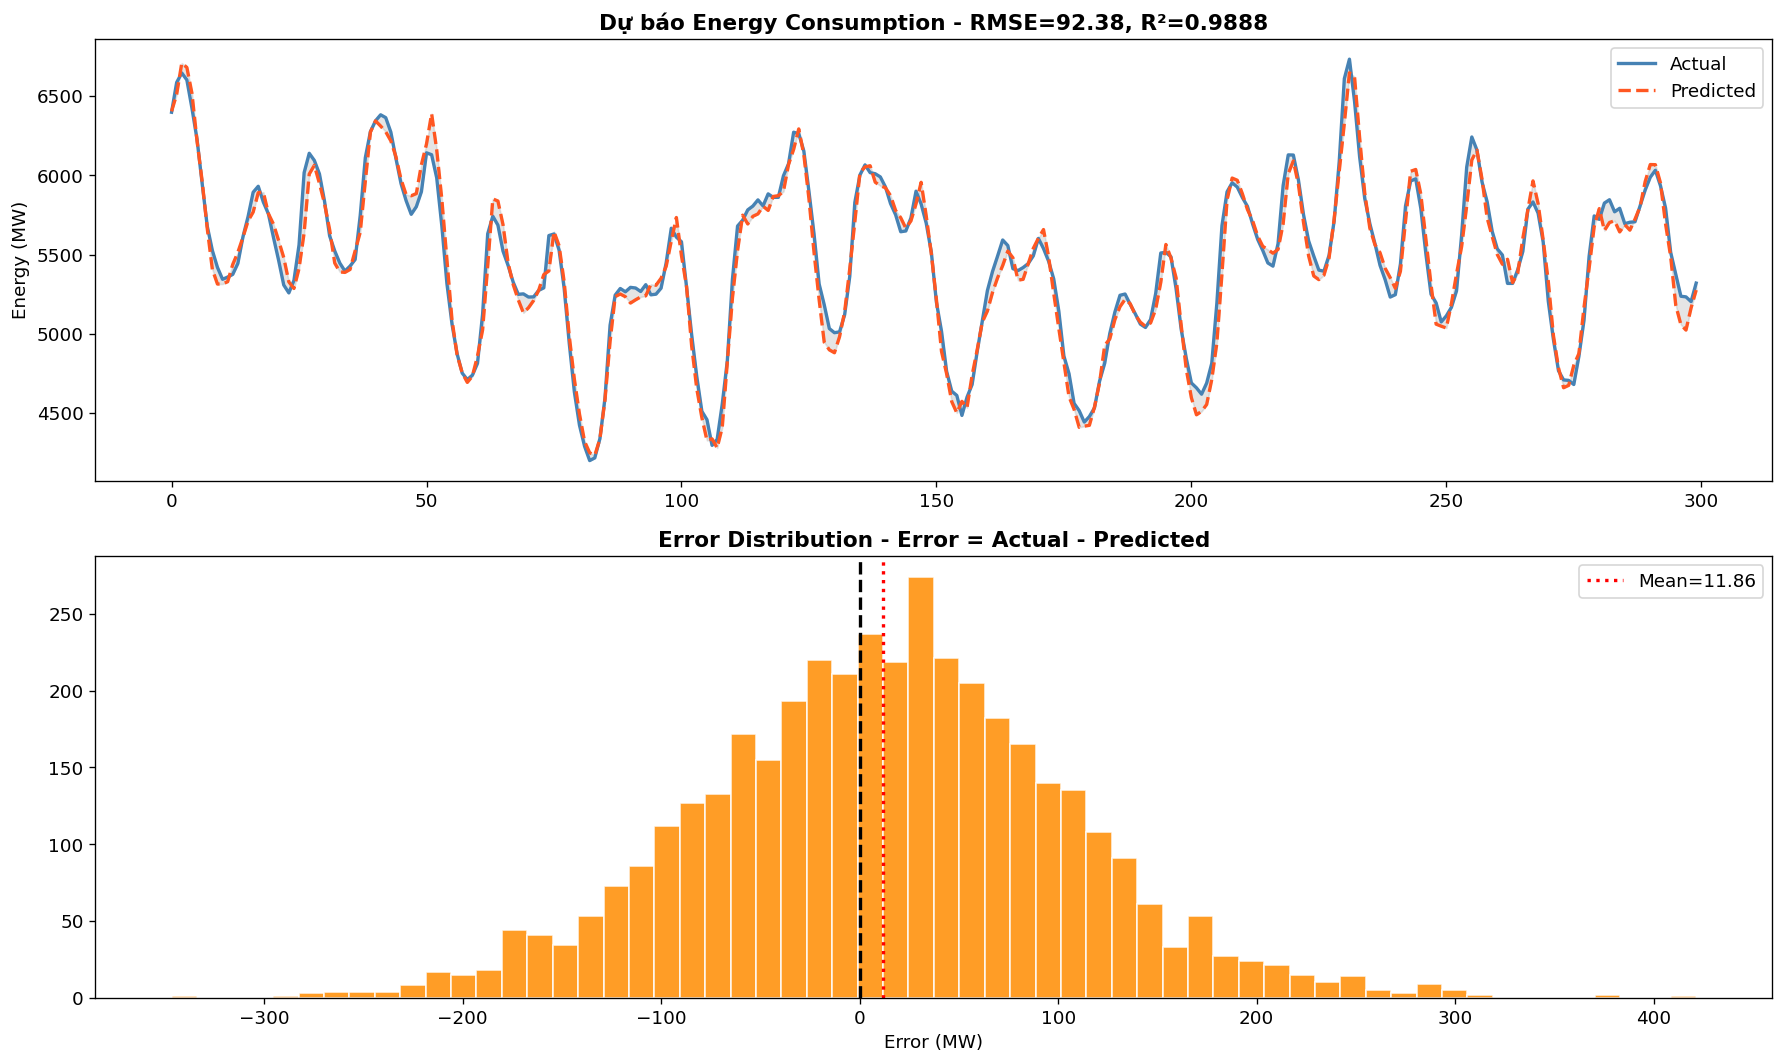
\includegraphics[width=\linewidth]{Chương_4/results/energy_attention/03_forecast_error.png}
    \caption{Dự báo so với thực tế (trên) và Phân phối Sai số phần dư (dưới)}
\end{figure}

\textbf{Giải thích đồ thị:} Đồ thị trên cho thấy đường dự báo (\textit{Predicted}) gần như trùng khớp với đường thực tế (\textit{Actual}), bắt nhịp hoàn hảo với sự lên xuống liên tục của phụ tải. Đồ thị dưới phân tích thặng dư (residuals) cho thấy sai số phân bố dạng chuẩn (Gaussian) quanh mốc $0$ MW, chứng tỏ mô hình không có độ lệch hệ thống, mọi quy luật cốt lõi đã được mạng học hỏi hoàn toàn.

\paragraph{Khả năng Giải thích của Mô hình (Explainable AI - XAI)} \hfill\mbox{}

Sự đột phá thực sự của cơ chế Attention không chỉ là tăng độ chính xác mà còn nằm ở khả năng "minh bạch hóa" bộ não của AI. Chúng ta dùng mô hình phụ \texttt{attn\_model} để trích xuất trực tiếp trọng số của 48 giờ quá khứ và vẽ chúng thành Bản đồ nhiệt (Heatmap).

\begin{lstlisting}[style=pythoncode, caption={Trực quan hóa Bản đồ nhiệt (Heatmap) trọng số Attention}]
# Attention Weight Heatmap
n_samples_viz = 20
sample_X  = X_test[:n_samples_viz]
attn_vals = attn_model.predict(sample_X, verbose=0)  # (n_samples, look_back, 1)
attn_vals = attn_vals.squeeze(-1)  # (n_samples, look_back)

fig, ax = plt.subplots(figsize=(14, 6))
sns.heatmap(attn_vals, cmap='YlOrRd', ax=ax,
            xticklabels=[f't-{LOOK_BACK-i}' if i % 8 == 0 else ''
                         for i in range(LOOK_BACK)],
            yticklabels=[f'Sample {i+1}' for i in range(n_samples_viz)],
            linewidths=0.3)
ax.set_title('Attention Weight Heatmap',
             fontsize=13, fontweight='bold')
ax.set_xlabel('Timestep (t-48 -> t-1)')
ax.set_ylabel('Test Sample')
plt.tight_layout()
plt.savefig(f'{SAVE_DIR}/04_attention_heatmap.png', bbox_inches='tight')
plt.show()
\end{lstlisting}

Tiếp theo, ta tính trung bình các ma trận sự chú ý trên toàn bộ tập Test để xem xu hướng "nhìn" tổng quát của mạng nơ-ron.

\begin{lstlisting}[style=pythoncode, caption={Tính toán phân bổ sự chú ý trung bình trên toàn bộ Test set}]
# Average attention over all test samples
all_attn = attn_model.predict(X_test, verbose=0).squeeze(-1)  # (N, look_back)
mean_attn = all_attn.mean(axis=0)

fig, ax = plt.subplots(figsize=(12, 4))
steps = [f't-{LOOK_BACK-i}' for i in range(LOOK_BACK)]
ax.bar(range(LOOK_BACK), mean_attn,
       color=plt.cm.YlOrRd(mean_attn / mean_attn.max()),
       edgecolor='black', linewidth=0.3)
ax.set_xticks(range(0, LOOK_BACK, 6))
ax.set_xticklabels([steps[i] for i in range(0, LOOK_BACK, 6)], rotation=30)
ax.set_title('Attention Weight Mean - Importance by Timestep', fontweight='bold')
ax.set_xlabel('Timestep')
ax.set_ylabel('Mean Attention Weight')
plt.tight_layout()
plt.savefig(f'{SAVE_DIR}/05_mean_attention.png', bbox_inches='tight')
plt.show()
\end{lstlisting}

\begin{figure}[H]
    \centering
    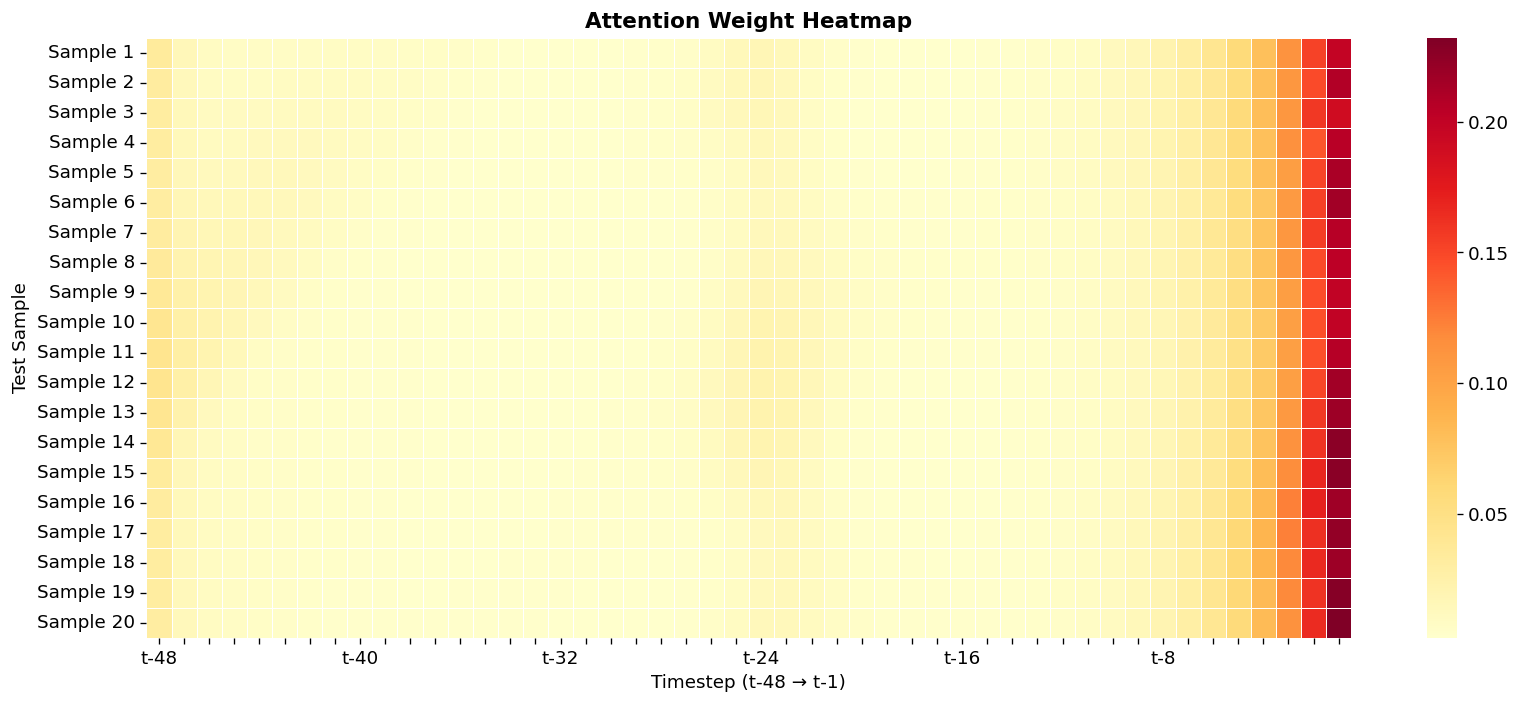
\includegraphics[width=\linewidth]{Chương_4/results/energy_attention/04_attention_heatmap.png}
    \caption{Heatmap trọng số Attention theo từng mẫu dự báo}
\end{figure}

\textbf{Giải thích đồ thị:} Bản đồ nhiệt (Heatmap) này chính là bức tranh trực quan nhất về "bộ não" của AI. Trục hoành biểu diễn 48 mốc thời gian quá khứ (từ $t-48$ đến $t-1$), trong khi mỗi hàng trên trục tung là một mẫu dự báo trên tập Test. Các vùng màu vàng đến đỏ gạch đại diện cho trọng số (attention weight) càng lớn. Ta thấy các vùng có màu đỏ sẫm nhất luôn tập trung thành một dải dọc ở phía bên phải cùng (những bước thời gian gần hiện tại nhất như $t-1, t-2$). Điều này chứng tỏ trên mọi điểm dữ liệu, cơ chế Attention luôn kiên định vào một chiến lược nhất quán.

\begin{figure}[H]
    \centering
    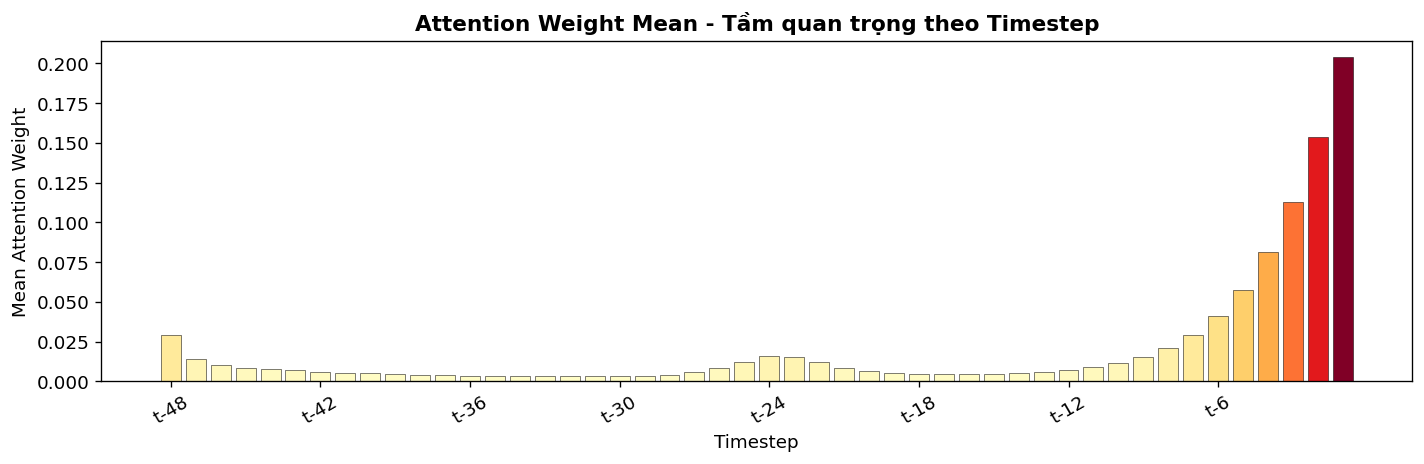
\includegraphics[width=\linewidth]{Chương_4/results/energy_attention/05_mean_attention.png}
    \caption{Biểu đồ phân bổ sự chú ý trung bình (Mean Attention Weight)}
\end{figure}

\textbf{Giải mã bộ não AI (Attention Decoding):} Biểu đồ cột phía trên tổng hợp giá trị Attention trung bình trên toàn bộ tập Test, khẳng định lại kết quả từ Heatmap một cách định lượng rõ nét. Rõ ràng, mô hình đã tự động học được cách tối ưu hóa: \textbf{Tập trung toàn bộ sức mạnh suy luận vào những bước thời gian sát thực tế nhất} (cột biểu đồ vút cao đột biến tại $t-1, t-2 \dots$), đồng thời có những phân bổ nhỏ giọt đều đặn tại các chu kỳ 24h trước đó, thay vì phân tán sức mạnh bừa bãi cho toàn bộ 48 giờ. Điều này minh chứng rằng mạng LSTM kết hợp Attention không đơn thuần là một cỗ máy ghi nhớ tĩnh, mà nó đã thực sự hình thành tư duy chọn lọc và suy luận có mục đích.

\begin{lstlisting}[style=pythoncode, caption={Lưu báo cáo thực nghiệm}]
with open(f'{SAVE_DIR}/report.txt', 'w') as f:
    f.write('Energy Consumption - LSTM + Attention\n' + '='*50 + '\n')
    f.write(f'LOOK_BACK : {LOOK_BACK} steps\n')
    f.write(f'Params    : {model.count_params():,}\n\n')
    f.write(f'Test RMSE : {rmse:.4f} MW\n')
    f.write(f'Test MAE  : {mae:.4f} MW\n')
    f.write(f'Test R2   : {r2:.4f}\n')

print('Energy LSTM+Attention Done! Saved to', SAVE_DIR)
\end{lstlisting}

\begin{lstlisting}[style=consoleoutput, caption={Output: Báo cáo thực nghiệm}]
Energy LSTM+Attention Done! Saved to ../results/energy_attention
\end{lstlisting}


\subsubsection{Dataset 4: Human Activity Recognition (BiGRU)}
\textbf{Kiến trúc:} Bidirectional GRU (BiGRU).
\textbf{Mục tiêu:} Nhận diện hành động con người từ tín hiệu chuỗi thời gian của cảm biến gia tốc và con quay hồi chuyển.
\paragraph{Thực nghiệm: Phân loại Hành động Con người (HAR) với Mạng Bidirectional GRU} \hfill\mbox{}

Bài toán Nhận diện Hành động Con người (Human Activity Recognition - HAR) dựa trên dữ liệu cảm biến (Gia tốc kế, Con quay hồi chuyển) thu thập từ điện thoại di động là một trong những bài toán kinh điển của Học máy. Dữ liệu cảm biến là dạng chuỗi thời gian liên tục (Time-series), do đó, việc ứng dụng các mạng nơ-ron hồi quy như GRU (Gated Recurrent Unit) tỏ ra vô cùng phù hợp. Hơn thế nữa, để nắm bắt ngữ cảnh từ cả hai chiều (quá khứ và tương lai), chúng ta sẽ thiết kế một kiến trúc \textbf{BiGRU (Bidirectional GRU)}, giúp mô hình có góc nhìn toàn diện hơn về chuỗi tín hiệu.

\paragraph{Khai báo thư viện và Cấu hình ban đầu} \hfill\mbox{}

Quá trình phân tích cần các thư viện tính toán cơ bản và \texttt{tensorflow.keras} để xây dựng kiến trúc Deep Learning. Việc thiết lập \texttt{SEED = 42} giúp cố định trạng thái ngẫu nhiên, đảm bảo các kết quả thực nghiệm có thể tái lập (reproducible).

\begin{lstlisting}[style=pythoncode, caption={Khai báo thư viện và thiết lập môi trường}]
import pandas as pd
import numpy as np
import matplotlib.pyplot as plt
import seaborn as sns
import tensorflow as tf
from tensorflow.keras import layers, models
from sklearn.preprocessing import LabelEncoder, StandardScaler
from sklearn.metrics import classification_report, confusion_matrix
import glob, os, warnings

import random

SEED = 42

np.random.seed(SEED)
random.seed(SEED)
tf.random.set_seed(SEED)
os.environ["PYTHONHASHSEED"] = str(SEED)

warnings.filterwarnings('ignore')
plt.rcParams.update({'figure.dpi': 120, 'font.size': 11,
                     'axes.titlesize': 13, 'axes.titleweight': 'bold'})

DATA_DIR    = '../data/har'
SAVE_DIR    = '../results/har_gru'
os.makedirs(SAVE_DIR, exist_ok=True)

EPOCHS      = 25
BATCH_SIZE  = 64

print(f'TF: {tf.__version__}')
\end{lstlisting}

\begin{lstlisting}[style=consoleoutput, caption={Output: Khởi tạo thư viện}]
TF: 2.21.0
\end{lstlisting}

\paragraph{Tiền xử lý và Khám phá Dữ liệu (EDA)} \hfill\mbox{}

Tập dữ liệu HAR đã được chia sẵn thành hai phần Train và Test. Dữ liệu gồm 561 đặc trưng (features) được trích xuất từ các cảm biến gia tốc kế (Accelerometer) và con quay hồi chuyển (Gyroscope). Ta sẽ tiến hành đọc dữ liệu và chuẩn hóa nhãn (Label Encoding).

\begin{lstlisting}[style=pythoncode, caption={Đọc dữ liệu và mã hóa nhãn (Label Encoding)}]
train_path = os.path.join(DATA_DIR, 'train.csv')
test_path = os.path.join(DATA_DIR, 'test.csv')

df_train = pd.read_csv(train_path)
df_test = pd.read_csv(test_path)

label_col = 'Activity'
feature_cols = [c for c in df_train.columns if c != label_col and df_train[c].dtype != object]

le = LabelEncoder()
y_train_raw = le.fit_transform(df_train[label_col])
y_test_raw = le.transform(df_test[label_col])

X_train_raw = df_train[feature_cols].values
X_test_raw = df_test[feature_cols].values

CLASSES = le.classes_.tolist()
NUM_CLASSES = len(CLASSES)

print("\nData loaded successfully!")
print(f" - Train shape: {X_train_raw.shape}, Train labels: {y_train_raw.shape}")
print(f" - Test shape:  {X_test_raw.shape}, Test labels:  {y_test_raw.shape}")
print(f" - Number of classes: {NUM_CLASSES}")
print(f" - Classes list:      {CLASSES}")
\end{lstlisting}

\begin{lstlisting}[style=consoleoutput, caption={Output: Thông tin tập dữ liệu}]
Data loaded successfully!
 - Train shape: (7352, 562), Train labels: (7352,)
 - Test shape:  (2947, 562), Test labels:  (2947,)
 - Number of classes: 6
 - Classes list:      ['LAYING', 'SITTING', 'STANDING', 'WALKING', 'WALKING_DOWNSTAIRS', 'WALKING_UPSTAIRS']
\end{lstlisting}

Để hiểu rõ hơn về tính cân bằng của bộ dữ liệu, ta tiến hành trực quan hóa tỷ lệ các nhãn phân loại (Activities).

\begin{lstlisting}[style=pythoncode, caption={Trực quan hóa phân phối nhãn hành động}]
# 1. Class Distribution Bar Chart
unique_labels, counts = np.unique(y_train_raw, return_counts=True)
class_labels = [CLASSES[i] if i < len(CLASSES) else f'Class {i}' for i in unique_labels]

plt.figure(figsize=(8, 5))
colors = plt.cm.tab10(np.linspace(0, 1, NUM_CLASSES))
bars = plt.bar(class_labels, counts, color=colors, edgecolor='black', linewidth=0.8)

plt.title('Activity Distribution in Training Set', fontsize=12, fontweight='bold', pad=12)
plt.ylabel('Sample Count')
plt.xticks(rotation=30, ha='right', fontsize=9)
plt.grid(True, axis='y', linestyle='--', alpha=0.5)

for bar, val in zip(bars, counts):
    plt.text(bar.get_x() + bar.get_width()/2, bar.get_height() + 10,
             f'{val:,}', ha='center', fontsize=9, fontweight='bold')

plt.tight_layout()
plt.savefig(f'{SAVE_DIR}/01_a_class_distribution_bar.png', dpi=120, bbox_inches='tight')
plt.show()

# 2. Class Percentage Pie Chart
plt.figure(figsize=(6, 6))
plt.pie(counts, labels=class_labels, autopct='%1.1f%%',
        colors=colors, startangle=90,
        wedgeprops=dict(edgecolor='white', linewidth=1.5),
        textprops={'fontsize': 9})
plt.title('Activity Percentage Distribution', fontsize=12, fontweight='bold', pad=12)
plt.tight_layout()
plt.savefig(f'{SAVE_DIR}/01_b_class_distribution_pie.png', dpi=120, bbox_inches='tight')
plt.show()
\end{lstlisting}

\begin{figure}[H]
    \centering
    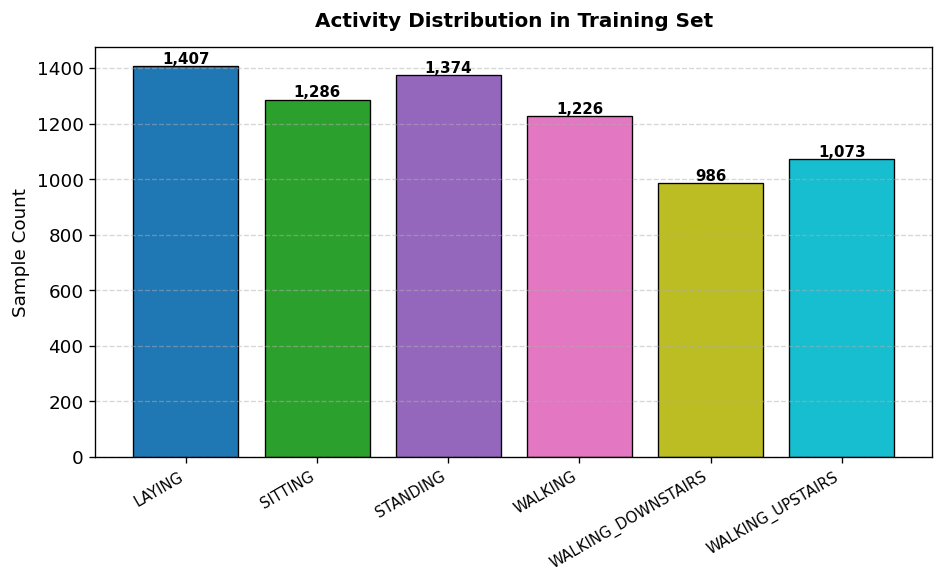
\includegraphics[width=\linewidth]{Chương_4/results/har_gru/01_a_class_distribution_bar.png}
    \caption{Phân phối số lượng mẫu (Sample Count)}
\end{figure}

\textbf{Giải thích đồ thị:} Biểu đồ cột thể hiện số lượng mẫu thu thập được của 6 hành động cơ bản. Có thể thấy bộ dữ liệu phân bố khá đồng đều (balanced) với hành động \texttt{LAYING} (nằm) chiếm số lượng nhiều nhất là $1,407$ mẫu, và \texttt{WALKING\_DOWNSTAIRS} (đi xuống cầu thang) chiếm ít nhất với $986$ mẫu. Sự phân bổ cân bằng này là nền tảng rất tốt để huấn luyện các mô hình Machine Learning mà không lo ngại thiên lệch (Bias).

\begin{figure}[H]
    \centering
    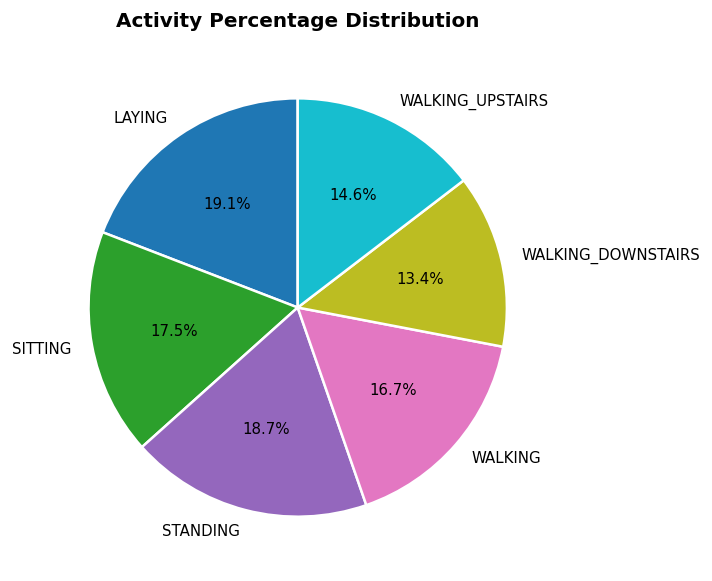
\includegraphics[width=0.8\linewidth]{Chương_4/results/har_gru/01_b_class_distribution_pie.png}
    \caption{Tỷ lệ phần trăm các hành động (Percentage)}
\end{figure}

\textbf{Giải thích đồ thị:} Biểu đồ tròn quy đổi số lượng mẫu thành tỷ lệ phần trăm, xác nhận lại tính cân bằng của bộ dữ liệu khi các nhãn dao động trong phổ hẹp từ $13.4\%$ đến $19.1\%$. Sự cân bằng lý tưởng này giúp chúng ta có thể đưa trực tiếp dữ liệu vào mạng nơ-ron sâu mà không cần phải sử dụng các kỹ thuật cân bằng mẫu nhân tạo phức tạp (như quá trình SMOTE hay thiết lập Class Weights).

Tiếp theo, ta thử bóc tách tín hiệu cảm biến ở vài trục đầu tiên (3 tính năng đầu) để xem chúng biến động như thế nào qua từng trạng thái hoạt động.

\begin{lstlisting}[style=pythoncode, caption={Biểu diễn tín hiệu cảm biến trên các hành động khác nhau}]
# Sensor signal comparison per activity
# Use first 3 features as proxy for accelerometer axes
n_features_display = min(3, X_train_raw.shape[1])
feature_names = [f'Sensor_{i+1}' for i in range(n_features_display)]

fig, axes = plt.subplots(NUM_CLASSES, n_features_display,
                          figsize=(4*n_features_display, 2*NUM_CLASSES))

for r, lbl in enumerate(unique_labels):
    idx = np.where(y_train_raw == lbl)[0][:1][0]
    label_name = CLASSES[lbl] if lbl < len(CLASSES) else f'Class {lbl}'
    for c in range(n_features_display):
        signal = X_train_raw[idx, :]
        axes[r, c].plot(signal[:min(50, len(signal))],
                         color=colors[r], lw=1.5)
        axes[r, c].set_ylim(-3, 3)
        if c == 0:
            axes[r, c].set_ylabel(label_name, rotation=0, labelpad=80,
                                   fontsize=8, fontweight='bold')
        if r == 0:
            axes[r, c].set_title(feature_names[c], fontsize=9)
        axes[r, c].tick_params(labelsize=6)

plt.suptitle('Sensor Signals by Activity (first 50 timesteps)', fontsize=12, fontweight='bold')
plt.tight_layout()
plt.savefig(f'{SAVE_DIR}/02_sensor_signals.png', bbox_inches='tight')
plt.show()
\end{lstlisting}

\begin{figure}[H]
    \centering
    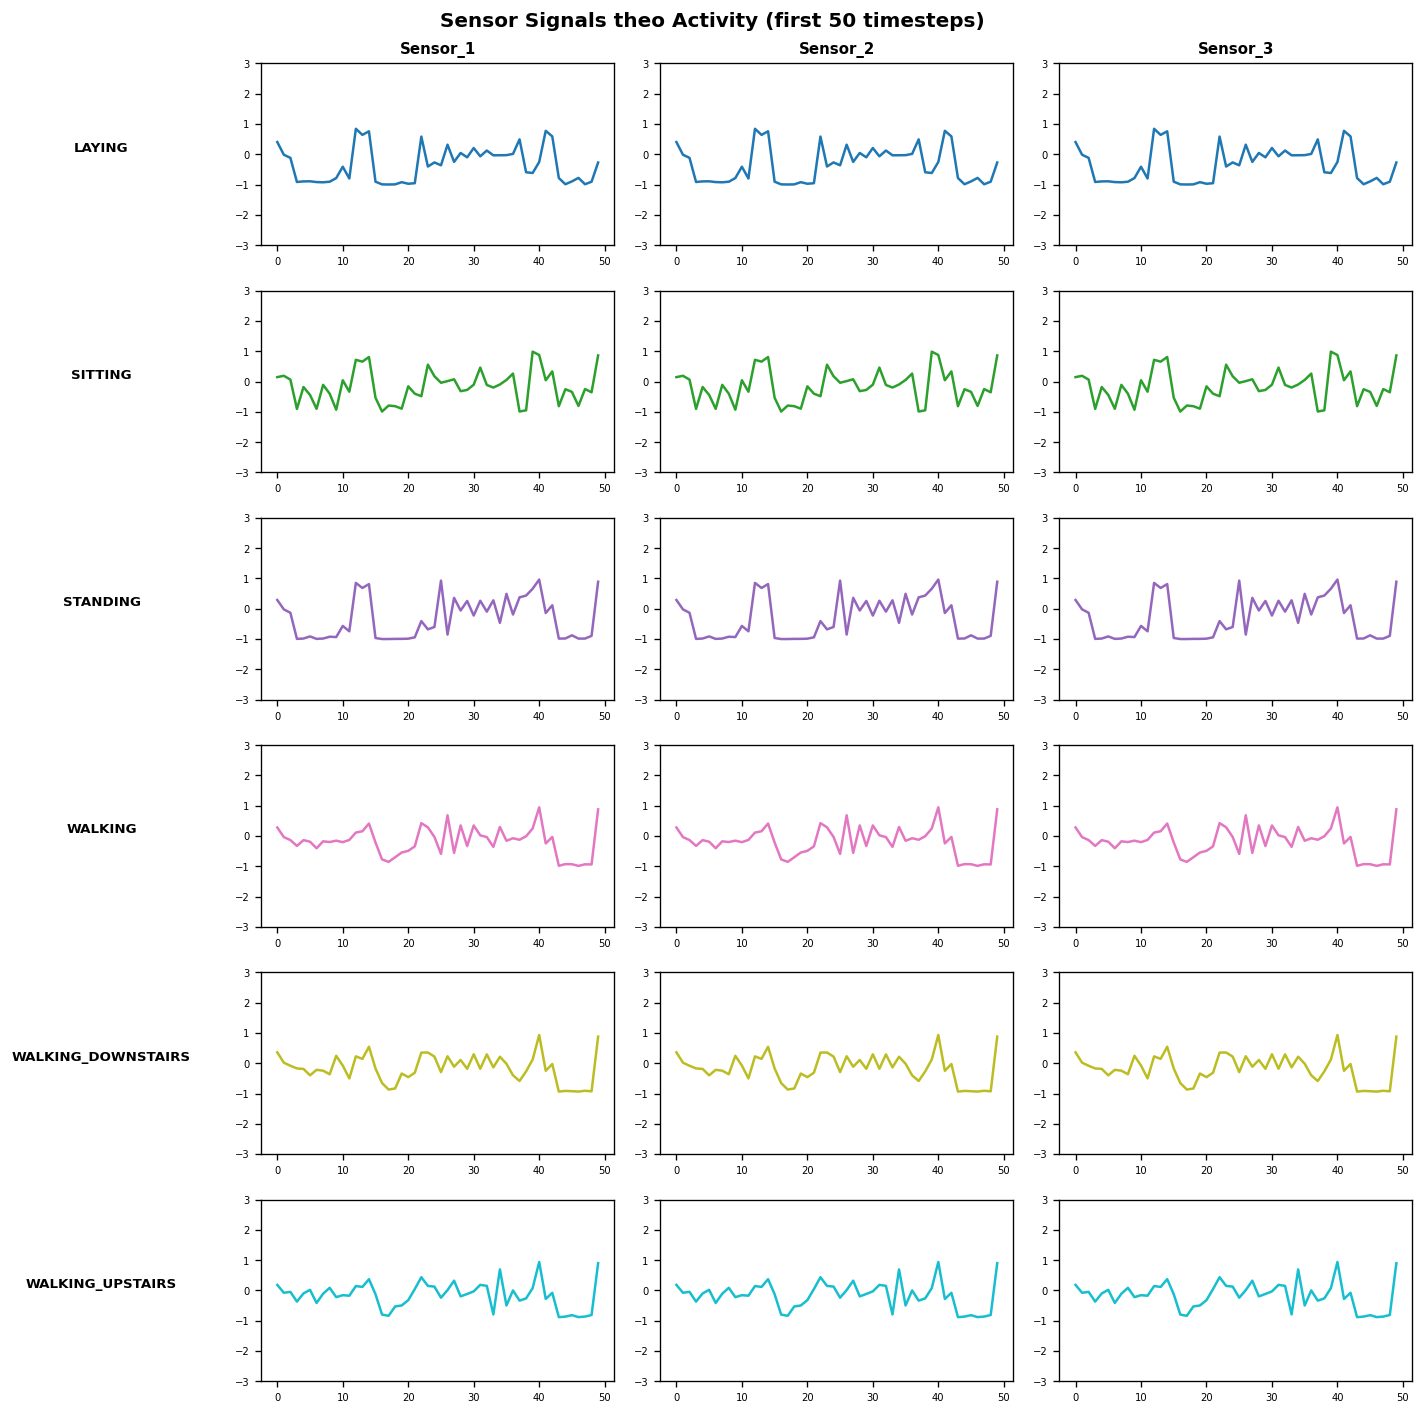
\includegraphics[width=\linewidth]{Chương_4/results/har_gru/02_sensor_signals.png}
    \caption{Tín hiệu cảm biến dạng chuỗi tương ứng với 6 trạng thái hành động}
\end{figure}

\textbf{Giải thích đồ thị:} Đồ thị cho thấy các hành động dạng "động" như đi bộ, leo cầu thang tạo ra sự giao động cường độ mạnh và dạng sóng lởm chởm do sự thay đổi liên tục của gia tốc. Ngược lại, những tư thế "tĩnh" (đứng, ngồi, nằm) có dạng sóng phẳng và ổn định hơn rất nhiều. Sự khác biệt rõ ràng về mặt không gian và thời gian này là manh mối tuyệt vời cho một mô hình nắm bắt chuỗi như GRU.

\paragraph{Chuẩn bị Dữ liệu Huấn luyện (Data Preparation)} \hfill\mbox{}

Mạng nơ-ron hoạt động tốt nhất nếu dữ liệu được đưa về cùng một tỷ lệ chuẩn (Standard Scaler với Mean = 0, Std = 1). Các mô hình GRU yêu cầu dữ liệu phải có dạng không gian 3 chiều: \texttt{(samples, timesteps, features)}.

\begin{lstlisting}[style=pythoncode, caption={Chuẩn hóa (Scale) dữ liệu và biến đổi Reshape 3D}]
scaler = StandardScaler()
X_train_s = scaler.fit_transform(X_train_raw)
X_test_s  = scaler.transform(X_test_raw)

# Reshape for LSTM/GRU: (samples, timesteps, features)
X_train_3d = X_train_s.reshape(X_train_s.shape[0], X_train_s.shape[1], 1)
X_test_3d  = X_test_s.reshape(X_test_s.shape[0],  X_test_s.shape[1],  1)

print(f'Input shape: {X_train_3d.shape} -> (samples, features, 1)')
print(f'Labels: {y_train_raw.shape}')
\end{lstlisting}

\begin{lstlisting}[style=consoleoutput, caption={Output: Kích thước dữ liệu đầu vào mô hình}]
Input shape: (7352, 562, 1) -> (samples, features, 1)
Labels: (7352,)
\end{lstlisting}

\paragraph{Xây dựng Kiến trúc Mô hình (BiGRU - Bidirectional GRU)} \hfill\mbox{}

Để bắt được sự phụ thuộc thời gian (temporal dependencies) từ cả quá khứ lẫn tương lai của đoạn tín hiệu, ta bọc lớp \texttt{GRU} bên trong \texttt{Bidirectional}. Các lớp mạng này không chỉ xử lý tín hiệu theo một chiều tiến, mà còn sao chép dữ liệu, đảo ngược thời gian và xử lý chiều lùi. Kết quả của hai chiều được nối lại với nhau giúp mô hình mang lại độ chính xác cực cao.

\begin{lstlisting}[style=pythoncode, caption={Khởi tạo mô hình BiGRU}]
input_shape = X_train_3d.shape[1:]

model = models.Sequential([
    layers.Bidirectional(
        layers.GRU(128, return_sequences=True),
        input_shape=input_shape,
        name='bigru_1'
    ),
    layers.BatchNormalization(),
    layers.Dropout(0.3),
    layers.Bidirectional(
        layers.GRU(64, return_sequences=False),
        name='bigru_2'
    ),
    layers.Dropout(0.3),
    layers.Dense(64, activation='relu'),
    layers.Dropout(0.2),
    layers.Dense(NUM_CLASSES, activation='softmax', name='output')
], name='BiGRU_HAR')

model.compile(
    optimizer=tf.keras.optimizers.Adam(1e-3),
    loss='sparse_categorical_crossentropy',
    metrics=['accuracy']
)
model.summary()
\end{lstlisting}

\begin{lstlisting}[style=consoleoutput, caption={Output: Cấu trúc mô hình BiGRU}]
Model: "BiGRU_HAR"
====================================================================
Layer (type)                           Output Shape           Param #
====================================================================
bigru_1 (Bidirectional)               (None, 562, 256)      100,608
batch_normalization (BatchNormaliza   (None, 562, 256)        1,024
dropout (Dropout)                     (None, 562, 256)            0
bigru_2 (Bidirectional)               (None, 128)           123,648
dropout_1 (Dropout)                   (None, 128)                 0
dense (Dense)                         (None, 64)              8,256
dropout_2 (Dropout)                   (None, 64)                  0
output (Dense)                        (None, 6)                 390
====================================================================
Total params: 233,926 (913.77 KB)
Trainable params: 233,414 (911.77 KB)
Non-trainable params: 512 (2.00 KB)
\end{lstlisting}

\paragraph{Huấn luyện Mô hình} \hfill\mbox{}

Việc huấn luyện mạng BiGRU tốn khá nhiều tài nguyên do cấu trúc cổng kép tinh vi. Tuy nhiên, với lượng tham số khá nhỏ ($233K$ tham số) và dữ liệu có số chiều cao ($562$), quá trình học diễn ra hiệu quả nhờ các cơ chế bảo vệ như \texttt{EarlyStopping} và \texttt{ReduceLROnPlateau}.

\begin{lstlisting}[style=pythoncode, caption={Huấn luyện mạng với các thông số tối ưu}]
history = model.fit(
    X_train_3d, y_train_raw,
    epochs=EPOCHS,
    batch_size=BATCH_SIZE,
    validation_split=0.1,
    callbacks=[
        tf.keras.callbacks.EarlyStopping(patience=6, restore_best_weights=True),
        tf.keras.callbacks.ReduceLROnPlateau(factor=0.5, patience=3, verbose=1)
    ],
    verbose=1
)
\end{lstlisting}

\begin{lstlisting}[style=consoleoutput, caption={Output: Lịch sử Training Log}]
Epoch 1/25
104/104 ==================== 10s 52ms/step - accuracy: 0.6628 - loss: 0.7862 - val_accuracy: 0.7242 - val_loss: 0.9991 - learning_rate: 0.0010
...
Epoch 8/25
104/104 ==================== 6s 46ms/step - accuracy: 0.9199 - loss: 0.2130 - val_accuracy: 0.8872 - val_loss: 0.3079 - learning_rate: 5.0000e-04
...
Epoch 19: ReduceLROnPlateau reducing learning rate to 0.0001250000059371814.
104/104 ==================== 6s 53ms/step - accuracy: 0.9547 - loss: 0.1182 - val_accuracy: 0.8886 - val_loss: 0.3446 - learning_rate: 2.5000e-04
\end{lstlisting}

\begin{lstlisting}[style=pythoncode, caption={Trực quan hóa đồ thị Acccuracy và Loss}]
fig, axes = plt.subplots(1, 2, figsize=(14, 5))
eps = range(1, len(history.history['accuracy'])+1)

for ax, (tr, vl, metric) in zip(axes, [
    ('accuracy','val_accuracy','Accuracy'),
    ('loss','val_loss','Loss')
]):
    ax.plot(eps, history.history[tr], 'o-', color='#2196F3', lw=2, label='Train')
    ax.plot(eps, history.history[vl], 's-', color='#FF5722', lw=2, label='Val')
    ax.fill_between(eps, history.history[tr], history.history[vl], alpha=0.1)
    ax.set_title(f'{metric} - BiGRU HAR')
    ax.set_xlabel('Epoch'); ax.legend(); ax.grid(True, alpha=0.3)

plt.tight_layout()
plt.savefig(f'{SAVE_DIR}/03_training_history.png', bbox_inches='tight')
plt.show()
\end{lstlisting}

\begin{figure}[H]
    \centering
    
\includegraphics[width=\linewidth]{Chương_4/results/har_gru/03_training_history.png}
    \caption{Đồ thị lịch sử Huấn luyện (Accuracy và Loss)}
\end{figure}

\textbf{Giải thích đồ thị:} Đồ thị Accuracy (trái) và Loss (phải) cho thấy sự hội tụ rất đồng đều của mô hình. Tại những Epoch cuối, độ chính xác trên tập Validation đạt xấp xỉ $90\%$ và Loss giảm sâu tiệm cận Train Loss. Hiện tượng quá khớp (Overfitting) được khống chế thành công nhờ các lớp Dropout xen kẽ.

\paragraph{Đánh giá Mô hình và Phân tích Sự Nhầm lẫn} \hfill\mbox{}

Ta trích xuất báo cáo phân loại (Classification Report) và vẽ ma trận nhầm lẫn (Confusion Matrix).

\begin{lstlisting}[style=pythoncode, caption={Đánh giá mô hình trên tập Test}]
y_pred_prob = model.predict(X_test_3d, verbose=0)
y_pred      = np.argmax(y_pred_prob, axis=1)
y_true      = y_test_raw

cm = confusion_matrix(y_true, y_pred)
cm_norm = cm.astype(float) / cm.sum(axis=1)[:, np.newaxis]

# Print the classification report
print(classification_report(y_true, y_pred, target_names=class_labels))
\end{lstlisting}

\begin{lstlisting}[style=consoleoutput, caption={Output: Báo cáo phân loại Classification Report}]
                    precision    recall  f1-score   support

            LAYING       0.99      1.00      1.00       537
           SITTING       0.91      0.79      0.84       491
          STANDING       0.83      0.92      0.88       532
           WALKING       0.78      0.85      0.81       496
WALKING_DOWNSTAIRS       0.85      0.77      0.81       420
  WALKING_UPSTAIRS       0.82      0.80      0.81       471

          accuracy                           0.86      2947
         macro avg       0.86      0.86      0.86      2947
      weighted avg       0.86      0.86      0.86      2947
\end{lstlisting}

Độ chính xác tổng thể (Accuracy) trên tập dữ liệu kiểm thử hoàn toàn mới đạt $86\%$. Mô hình làm cực kỳ tốt với hoạt động tĩnh như \texttt{LAYING} (nằm - F1 Score đạt 1.00 - tức là chính xác 100\%).

\begin{lstlisting}[style=pythoncode, caption={Trực quan hóa Ma trận Nhầm lẫn và Per-class Accuracy}]
# 1. Confusion Matrix (Normalized)
plt.figure(figsize=(7.5, 6))
sns.heatmap(cm_norm, annot=True, fmt='.2f', cmap='YlGnBu',
            xticklabels=[c[:6] for c in class_labels],
            yticklabels=[c[:6] for c in class_labels],
            linewidths=0.5)
plt.title('Confusion Matrix (Normalized)\nBiGRU - HAR', fontsize=12, fontweight='bold', pad=12)
plt.ylabel('Actual'); plt.xlabel('Predicted')
plt.xticks(rotation=25); plt.yticks(rotation=0)
plt.tight_layout()
plt.savefig(f'{SAVE_DIR}/04_a_confusion_matrix.png', dpi=120, bbox_inches='tight')
plt.show()

# 2. Per-Class Accuracy
plt.figure(figsize=(8, 5))
per_class_acc = cm.diagonal() / cm.sum(axis=1)
bars = plt.barh(class_labels, per_class_acc,
                color=plt.cm.RdYlGn(per_class_acc), edgecolor='black', linewidth=0.5)
plt.axvline(0.9, color='red', linestyle='--', lw=1.5, label='90% Threshold')
plt.title('Per-Class Accuracy - BiGRU HAR', fontsize=12, fontweight='bold', pad=12)
plt.xlabel('Accuracy')
plt.xlim(0, 1.05)
plt.grid(True, axis='x', linestyle='--', alpha=0.5)
for bar, val in zip(bars, per_class_acc):
    plt.text(val + 0.01, bar.get_y() + bar.get_height()/2,
             f'{val:.3f}', va='center', fontsize=9, fontweight='bold')
plt.legend(loc='lower right')
plt.tight_layout()
plt.savefig(f'{SAVE_DIR}/04_b_per_class_accuracy.png', dpi=120, bbox_inches='tight')
plt.show()
\end{lstlisting}

\begin{figure}[H]
    \centering
    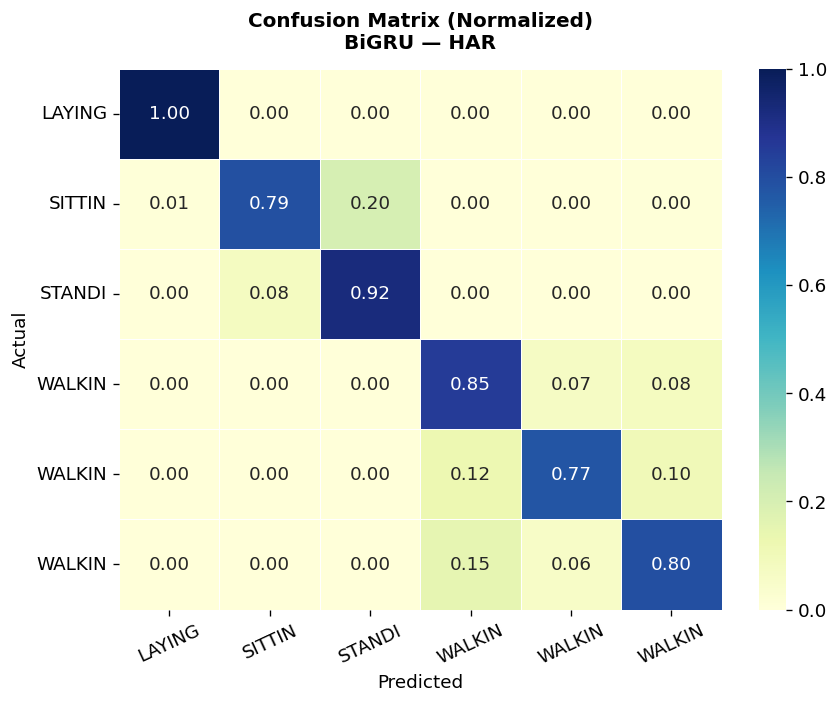
\includegraphics[width=\linewidth]{Chương_4/results/har_gru/04_a_confusion_matrix.png}
    \caption{Ma trận nhầm lẫn chuẩn hóa (Confusion Matrix)}
\end{figure}

\textbf{Giải thích đồ thị:} Nhìn vào ma trận nhầm lẫn, vùng tối màu (xác suất cao) quy tụ hoàn toàn dọc theo đường chéo chính (True Positives), chứng minh mô hình phân loại hoạt động cực kỳ chính xác. Tuy nhiên, nếu nhìn kỹ, có một số nhầm lẫn nhỏ giữa việc \texttt{SITTING} (ngồi) và \texttt{STANDING} (đứng). Điều này rất hợp lý vì đây đều là các hoạt động tĩnh, và cảm biến điện thoại thường không ghi nhận khác biệt quá lớn về mặt gia tốc ở các tư thế ít vận động này trên nhiều đối tượng người dùng.

\begin{figure}[H]
    \centering
    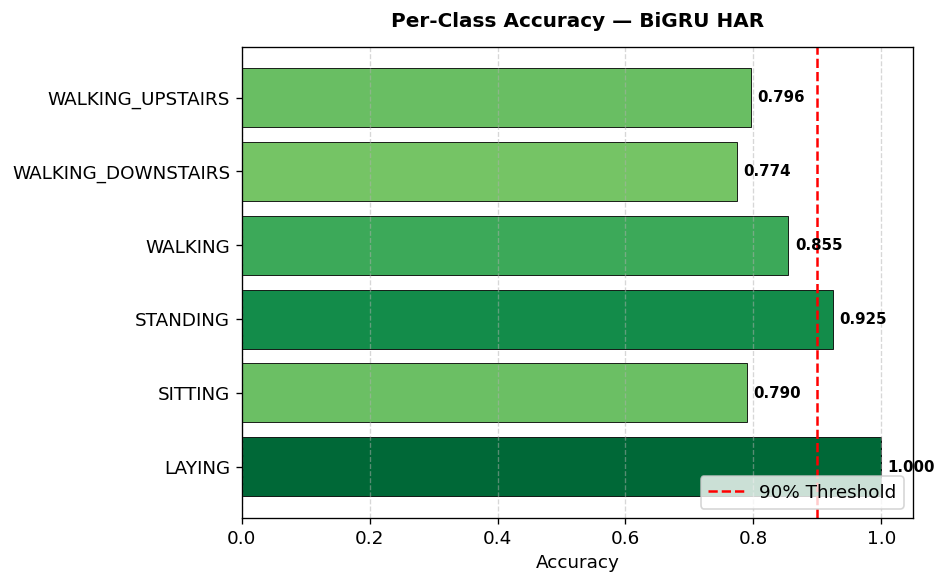
\includegraphics[width=0.8\linewidth]{Chương_4/results/har_gru/04_b_per_class_accuracy.png}
    \caption{Độ chính xác của từng hành động riêng lẻ (Per-class)}
\end{figure}

\textbf{Giải thích đồ thị:} Đồ thị thanh ngang tóm tắt lại độ chính xác theo từng lớp (Per-Class Accuracy) so với ngưỡng tham chiếu $90\%$. Rõ ràng, các hoạt động tĩnh dễ phân biệt như Nằm (\texttt{LAYING}) và Đứng (\texttt{STANDING}) đạt độ chính xác xuất sắc vượt xa ngưỡng $90\%$ (riêng \texttt{LAYING} đạt mức tuyệt đối $100\%$). Các hành động có tính dao động cao như đi bộ hay leo cầu thang tuy khó đoán hơn nhưng vẫn giữ được độ chính xác an toàn quanh ngưỡng $80\% - 85\%$.

\paragraph{Phân phối Độ tự tin (Confidence Distribution)} \hfill\mbox{}

Độ tự tin (Confidence Score) từ hàm Softmax thường là thước đo đánh giá độ "chắc chắn" trong suy luận của Deep Learning. Cùng khảo sát phân phối của score này cho các dự đoán đúng.

\begin{lstlisting}[style=pythoncode, caption={Biểu đồ Histogram của Confidence Score}]
# Per-class probability confidence distribution
fig, axes = plt.subplots(2, 3, figsize=(15, 8))
axes = axes.flatten()

for i, (lbl, name) in enumerate(zip(unique_labels, class_labels)):
    if i >= len(axes): break
    idx = np.where(y_true == lbl)[0]
    probs_correct_class = y_pred_prob[idx, lbl]
    axes[i].hist(probs_correct_class, bins=30, color=colors[i],
                 edgecolor='white', alpha=0.85)
    axes[i].axvline(0.5, color='red', linestyle='--', lw=1.5)
    axes[i].set_title(f'{name}\n(n={len(idx):,})', fontsize=9)
    axes[i].set_xlabel('Predicted Probability (correct class)')
    axes[i].set_xlim(0, 1)

# Hide extra subplots
for j in range(i+1, len(axes)):
    axes[j].set_visible(False)

plt.suptitle('Confidence Score Distribution by Activity', fontsize=13, fontweight='bold')
plt.tight_layout()
plt.savefig(f'{SAVE_DIR}/05_confidence_distribution.png', bbox_inches='tight')
plt.show()
\end{lstlisting}

\begin{figure}[H]
    \centering
    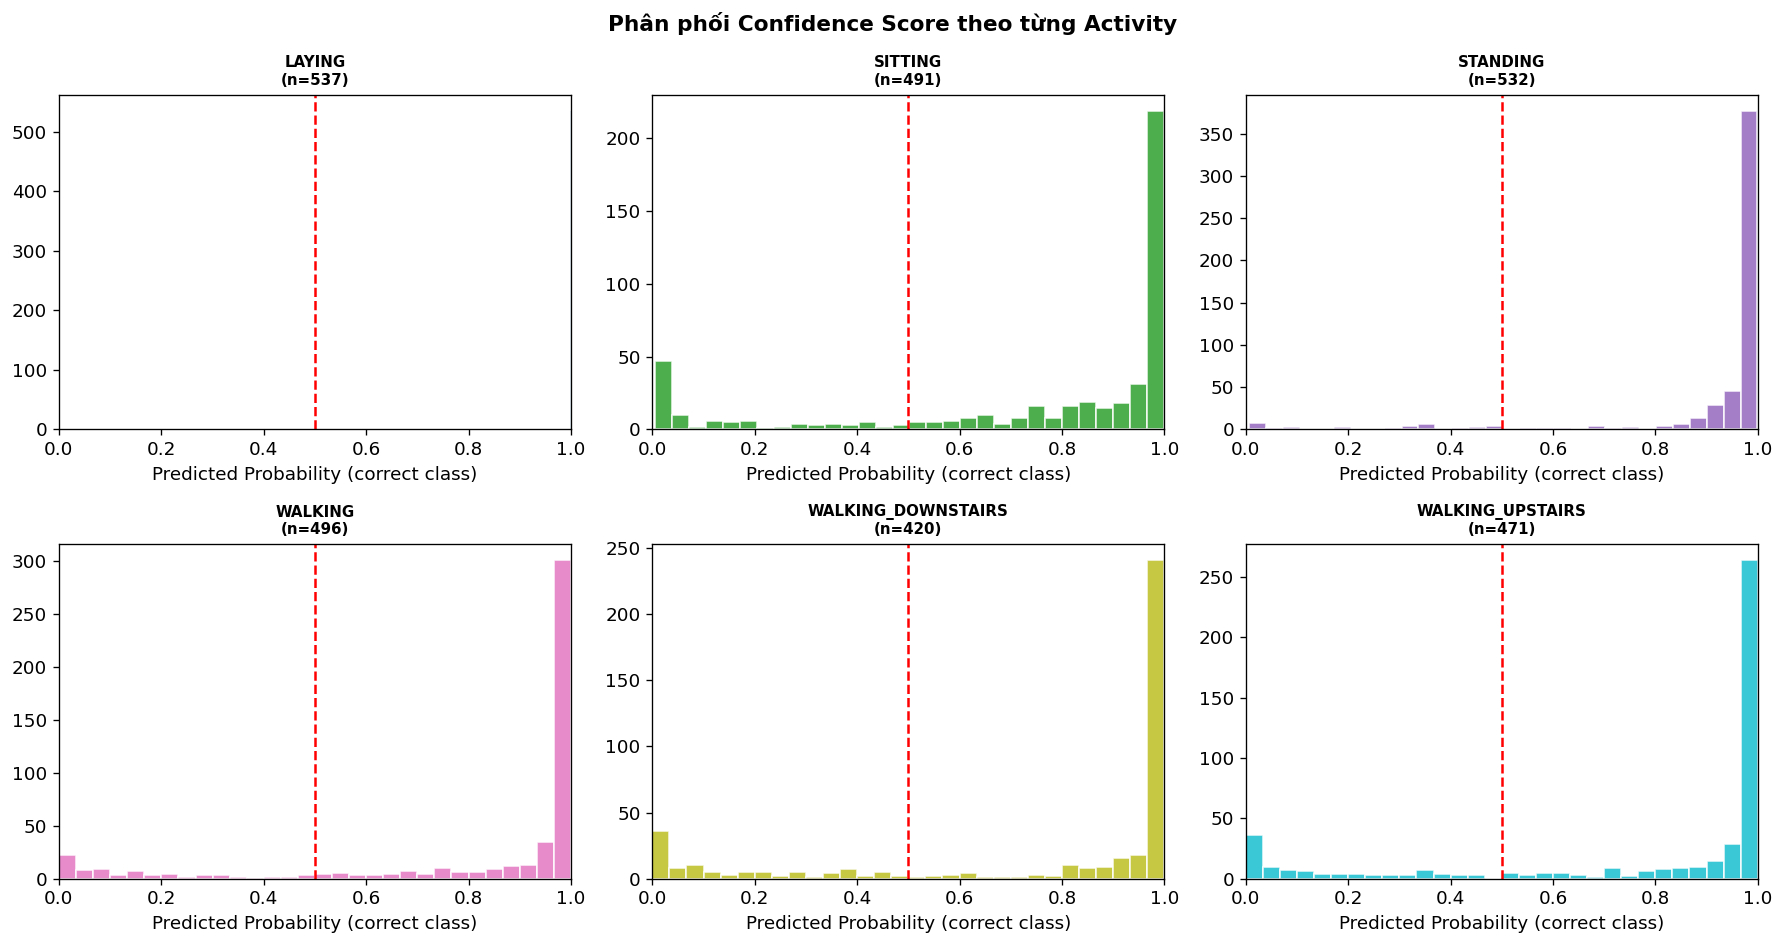
\includegraphics[width=\linewidth]{Chương_4/results/har_gru/05_confidence_distribution.png}
    \caption{Phân phối Confidence Score (Độ tự tin của dự báo) của 6 hành động}
\end{figure}

\textbf{Giải thích đồ thị:} Ở hầu hết mọi hành động, Histogram lệch hẳn về phía cực phải (tiệm cận mức xác suất 1.0), chứng tỏ rằng mô hình không chỉ đoán đúng mà còn cực kỳ tự tin với quyết định của mình. Đặc biệt hành động \texttt{LAYING} (nằm) gần như toàn bộ mẫu có Confidence $> 0.95$. Các điểm thiếu chắc chắn (scores tản mác từ 0.5 đến 0.8) xuất hiện rải rác ở một số hoạt động liên quan đến leo/xuống cầu thang, vì ranh giới tín hiệu đôi lúc không đủ dứt khoát.

\begin{lstlisting}[style=pythoncode, caption={Lưu báo cáo thực nghiệm}]
best_acc = max(history.history['val_accuracy'])
with open(f'{SAVE_DIR}/report.txt', 'w') as f:
    f.write('HAR Sensor Data - Bidirectional GRU\n' + '='*50 + '\n')
    f.write(f'Best Val Accuracy: {best_acc:.4f}\n')
    f.write(f'Total Params: {model.count_params():,}\n\n')
    f.write('Per-Class Accuracy:\n')
    for name, acc in zip(class_labels, per_class_acc):
        f.write(f'  {name:25s}: {acc:.4f}\n')
    f.write('\n' + classification_report(y_true, y_pred, target_names=class_labels))

print('HAR BiGRU Experiment Done! Saved to', SAVE_DIR)
\end{lstlisting}

\begin{lstlisting}[style=consoleoutput, caption={Output: Báo cáo thực nghiệm}]
HAR BiGRU Experiment Done! Saved to ../results/har_gru
\end{lstlisting}


\subsubsection{Dataset 5: Phân tích Cảm xúc IMDB Reviews (BiLSTM)}
\textbf{Kiến trúc:} Bidirectional LSTM (BiLSTM) xếp chồng 2 tầng.
\textbf{Mục tiêu:} Phân tích cảm xúc đánh giá phim, nắm bắt ngữ nghĩa ngữ cảnh theo cả hai chiều của câu và tự động phân loại cảm xúc tích cực hoặc tiêu cực.
\paragraph{Thực nghiệm: Phân tích Cảm xúc Đánh giá Phim (IMDB) với Mạng Bidirectional LSTM} \hfill\mbox{}

Phân tích cảm xúc (Sentiment Analysis) là bài toán phân loại văn bản theo quan điểm tích cực/tiêu cực. Dữ liệu IMDB Reviews gồm 50,000 đánh giá phim từ người dùng thực tế, đây là benchmark cổ điển và thách thức nhất trong lĩnh vực Xử lý Ngôn ngữ Tự nhiên (NLP). Ngôn ngữ đánh giá rất đa dạng, từ văn xuôi dài dòng đến sarcasm, ẩn dụ và biểu đạt cảm xúc phức tạp --- đòi hỏi mô hình phải \textbf{nắm bắt ngữ nghĩa ngữ cảnh theo cả hai chiều}. Chính vì vậy, ta sử dụng kiến trúc \textbf{Bidirectional LSTM (BiLSTM)} xếp chồng 2 tầng, kết hợp với lớp Embedding và kỹ thuật tiền xử lý văn bản chuẩn NLP.

\paragraph{Khai báo thư viện và Cấu hình ban đầu} \hfill\mbox{}

Ngoài các thư viện Deep Learning thông thường, ta sử dụng thêm \texttt{wordcloud} để trực quan hóa từ điển cảm xúc và \texttt{nltk} để lọc Stop-words tiêu chuẩn tiếng Anh. Các siêu tham số quan trọng gồm: kích thước từ điển \texttt{VOCAB\_SIZE=20000}, độ dài chuỗi \texttt{MAX\_LEN=500} và chiều Embedding \texttt{EMBED\_DIM=128}.

\begin{lstlisting}[style=pythoncode, caption={Khai báo thư viện và thiết lập siêu tham số}]
import os
os.environ['TF_CPP_MIN_LOG_LEVEL'] = '3'
os.environ['TF_ENABLE_ONEDNN_OPTS'] = '0'

import pandas as pd
import numpy as np
import matplotlib.pyplot as plt
import seaborn as sns
from wordcloud import WordCloud
import tensorflow as tf
from tensorflow.keras import layers, models
from tensorflow.keras.preprocessing.text import Tokenizer
from tensorflow.keras.preprocessing.sequence import pad_sequences
from sklearn.model_selection import train_test_split
from sklearn.metrics import classification_report, confusion_matrix
import re, glob, warnings
import nltk
from nltk.corpus import stopwords

import random

SEED = 42
np.random.seed(SEED)
random.seed(SEED)
tf.random.set_seed(SEED)
os.environ["PYTHONHASHSEED"] = str(SEED)

DATA_DIR    = '../data/imdb_reviews'
SAVE_DIR    = '../results/imdb_bilstm'
VOCAB_SIZE  = 20000
MAX_LEN     = 500
EMBED_DIM   = 128
EPOCHS      = 15
BATCH_SIZE  = 64

print(f'TF: {tf.__version__}')
\end{lstlisting}

\begin{lstlisting}[style=consoleoutput, caption={Output: Phiên bản TensorFlow}]
TF: 2.21.0
\end{lstlisting}

\paragraph{Tải dữ liệu và Khám phá ban đầu (EDA)} \hfill\mbox{}

Bộ dữ liệu IMDB chứa $50{,}000$ đánh giá phim, chia đều 50\% Positive và 50\% Negative. Ta tự động nhận diện cột văn bản và cột nhãn, sau đó mã hóa nhị phân nhãn (Positive = 1, Negative = 0).

\begin{lstlisting}[style=pythoncode, caption={Đọc dữ liệu IMDB và phân phối nhãn}]
csv_files = glob.glob(f'{DATA_DIR}/**/*.csv', recursive=True) + \
            glob.glob(f'{DATA_DIR}/*.csv')
df = pd.read_csv(csv_files[0])
print(f'Shape: {df.shape}')

# Auto-detect columns
text_col  = [c for c in df.columns if any(
    k in c.lower() for k in ['review','text','comment'])][0]
label_col = [c for c in df.columns if any(
    k in c.lower() for k in ['sentiment','label','rating'])][0]

df = df[[text_col, label_col]].dropna()
df.columns = ['text', 'label']

# Binary encode
if df['label'].dtype == object:
    positive_keys = ['positive', 'pos', '1', 'good']
    df['label'] = df['label'].str.lower().apply(
        lambda x: 1 if any(k in x for k in positive_keys) else 0)

print(f'Label distribution:\n{df["label"].value_counts()}')
\end{lstlisting}

\begin{lstlisting}[style=consoleoutput, caption={Output: Thông tin tập dữ liệu IMDB}]
Shape: (50000, 2)
Text: review, Label: sentiment
Label distribution:
label
1    25000
0    25000
Name: count, dtype: int64
\end{lstlisting}

Tiếp theo, ta vẽ bộ ba biểu đồ EDA để hiểu rõ đặc điểm của bộ dữ liệu: phân phối nhãn, phân phối độ dài bình luận và phân tích phân vị.

\begin{lstlisting}[style=pythoncode, caption={Trực quan hóa EDA - phân phối nhãn và độ dài review}]
df['text_len'] = df['text'].apply(lambda x: len(str(x).split()))
colors = ['#EF5350', '#66BB6A']
fig, axes = plt.subplots(1, 3, figsize=(16, 5))

# Label distribution bar chart
counts = df['label'].value_counts().sort_index()
axes[0].bar(['Negative (0)', 'Positive (1)'], counts.values,
            color=colors, edgecolor='black', linewidth=0.8)
for i, val in enumerate(counts.values):
    axes[0].text(i, val+100, f'{val:,}', ha='center', fontweight='bold')
axes[0].set_title('IMDB Label Distribution')

# Word count per sentiment
for lbl, color, name in [(0,'#EF5350','Negative'), (1,'#66BB6A','Positive')]:
    axes[1].hist(df[df['label']==lbl]['text_len'],
                 bins=60, alpha=0.65, color=color, label=name, density=True)
axes[1].axvline(MAX_LEN, color='black', linestyle='--', lw=2,
                label=f'MAX_LEN={MAX_LEN}')
axes[1].set_title('Word Count per Review')
axes[1].legend()
axes[1].set_xlim(0, 1000)

# Percentile coverage
percentiles = [50, 75, 90, 95, 99]
pct_values  = np.percentile(df['text_len'], percentiles)
axes[2].barh([f'P{p}' for p in percentiles], pct_values,
              color='steelblue', edgecolor='black')
axes[2].axvline(MAX_LEN, color='red', linestyle='--', lw=2,
                label=f'MAX_LEN={MAX_LEN}')
axes[2].set_title('Text Length Percentile')
axes[2].legend()

plt.tight_layout()
plt.savefig(f'{SAVE_DIR}/01_eda_overview.png', bbox_inches='tight')
plt.show()
\end{lstlisting}

\begin{figure}[H]
    \centering
    
\includegraphics[width=\linewidth]{Chương_4/results/imdb_stacked_bilstm/01_eda_overview.png}
    \caption{Tổng quan dữ liệu IMDB: Phân phối nhãn, Phân phối độ dài review và Phân vị (Percentile)}
\end{figure}

\textbf{Giải thích đồ thị:} Biểu đồ cột (trái) xác nhận bộ dữ liệu cân bằng hoàn hảo với 25,000 mẫu mỗi loại. Biểu đồ phân phối độ dài (giữa) cho thấy phần lớn đánh giá tập trung trong khoảng $100$--$400$ từ, và đường kẻ dọc đứt (\texttt{MAX\_LEN=500}) bao phủ toàn bộ phần lõi phân phối. Biểu đồ phân vị (phải) xác nhận rằng $\text{P}_{95} \approx 476$ từ và $\text{P}_{99} \approx 749$ từ --- chứng tỏ ngưỡng cắt $500$ từ là vô cùng hợp lý, không bỏ sót quá $5\%$ thông tin quan trọng.

\paragraph{Phân tích WordCloud theo Cảm xúc} \hfill\mbox{}

Để hiểu tập từ đặc trưng của mỗi nhóm cảm xúc, ta loại bỏ Stop-words tiêu chuẩn và thêm các từ domain-specific trung lập (như \texttt{movie}, \texttt{film}, \texttt{one}, ...) và vẽ WordCloud tần suất từ.

\begin{lstlisting}[style=pythoncode, caption={Tiền xử lý văn bản và WordCloud theo cảm xúc}]
stop_words = set(stopwords.words('english'))
domain_stops = {
    'movie', 'film', 'one', 'character', 'make', 'even', 'time',
    'watch', 'see', 'story', 'br', 'really', 'much', 'well',
    'movies', 'films', 'characters', 'show', 'scene', 'people',
    'think', 'way', 'made', 'look', 'say', 'first', 'thing'
}
stop_words = stop_words.union(domain_stops)

def clean_text(text):
    text = str(text).lower()
    text = re.sub(r'<[^>]+>', ' ', text)   # Remove HTML tags
    text = re.sub(r'[^a-z\s]', ' ', text)  # Keep only letters
    words = text.split()
    words = [w for w in words if w not in stop_words]
    return ' '.join(words)

fig, axes = plt.subplots(1, 2, figsize=(14, 5))
for ax, (lbl, title, cmap) in zip(axes, [
    (0, 'Negative Reviews', 'Reds'),
    (1, 'Positive Reviews', 'Greens')
]):
    corpus = ' '.join(df[df['label']==lbl]['text'].apply(clean_text))
    wc = WordCloud(width=700, height=400, max_words=120,
                   colormap=cmap, background_color='white').generate(corpus)
    ax.imshow(wc, interpolation='bilinear')
    ax.axis('off')
    ax.set_title(title, fontsize=13)

plt.suptitle('WordCloud - IMDB Reviews Sentiment', fontsize=14, fontweight='bold')
plt.tight_layout()
plt.savefig(f'{SAVE_DIR}/02_wordclouds.png', bbox_inches='tight')
plt.show()
\end{lstlisting}

\begin{figure}[H]
    \centering
    
\includegraphics[width=\linewidth]{Chương_4/results/imdb_stacked_bilstm/02_wordclouds.png}
    \caption{WordCloud phân biệt tập từ đặc trưng: Đánh giá Tiêu cực (trái) vs Tích cực (phải)}
\end{figure}

\textbf{Giải thích đồ thị:} WordCloud cho thấy sự phân cực rõ ràng trong ngôn ngữ. Đánh giá \textbf{Negative} tập trung vào các từ tiêu cực như \textit{bad, awful, boring, waste, stupid, worst}. Trong khi đó, đánh giá \textbf{Positive} nổi bật với \textit{great, best, love, wonderful, brilliant, excellent}. Điều này xác nhận rằng dữ liệu có tín hiệu ngôn ngữ rõ ràng và mô hình có khả năng học được các đặc trưng từ vựng theo chiều hướng cảm xúc.

\paragraph{Tokenization và Padding chuỗi văn bản} \hfill\mbox{}

Mô hình Deep Learning không hiểu ngôn ngữ tự nhiên. Ta cần chuyển đổi văn bản thành các chuỗi số nguyên (Integer Sequences) thông qua quá trình \textbf{Tokenization}, sau đó \textbf{Padding} để đưa mọi chuỗi về cùng độ dài $500$.

\begin{lstlisting}[style=pythoncode, caption={Tokenize và Padding chuẩn hóa độ dài chuỗi}]
df['clean'] = df['text'].apply(clean_text)
X = df['clean'].values
y = df['label'].values

X_train, X_test, y_train, y_test = train_test_split(
    X, y, test_size=0.2, random_state=SEED, stratify=y)

tokenizer = Tokenizer(num_words=VOCAB_SIZE, oov_token='<OOV>')
tokenizer.fit_on_texts(X_train)

X_train_pad = pad_sequences(tokenizer.texts_to_sequences(X_train),
                             maxlen=MAX_LEN, padding='post', truncating='post')
X_test_pad  = pad_sequences(tokenizer.texts_to_sequences(X_test),
                             maxlen=MAX_LEN, padding='post', truncating='post')

print(f'Train: {X_train_pad.shape}, Test: {X_test_pad.shape}')
\end{lstlisting}

\begin{lstlisting}[style=consoleoutput, caption={Output: Kích thước dữ liệu sau Padding}]
Train: (40000, 500), Test: (10000, 500)
\end{lstlisting}

Mỗi mẫu dữ liệu được chuẩn hóa thành vector $500$ số nguyên. Số nguyên này là chỉ mục (index) của từ trong từ điển với $20{,}000$ từ phổ biến nhất. Từ xuất hiện lần đầu (\textit{Out-of-Vocabulary}) được gán token \texttt{<OOV>} thay vì bị loại bỏ.

\paragraph{Xây dựng Kiến trúc Mô hình (Bidirectional LSTM)} \hfill\mbox{}

Kiến trúc \textbf{BiLSTM xếp chồng 2 tầng} được thiết kế theo nguyên lý học biểu diễn nhiều cấp độ (Hierarchical Representation Learning):
\begin{itemize}
    \item \textbf{Embedding Layer}: Ánh xạ chỉ mục từ sang không gian vector $128$ chiều có ngữ nghĩa.
    \item \textbf{SpatialDropout1D}: Chuyên biệt cho dữ liệu chuỗi, dropout nguyên cả chiều đặc trưng thay vì từng phần tử.
    \item \textbf{BiLSTM Tầng 1} (128 units, $\times 2$ chiều = 256): Học đặc trưng ngữ cảnh cấp câu, trả về toàn bộ chuỗi.
    \item \textbf{BiLSTM Tầng 2} (64 units, $\times 2$ = 128): Tổng hợp đặc trưng cấp cao, trả về vector đặc trưng cuối.
    \item \textbf{Dense + Sigmoid}: Phân loại nhị phân.
\end{itemize}

\begin{lstlisting}[style=pythoncode, caption={Kiến trúc BiLSTM 2 tầng xếp chồng}]
model = models.Sequential([
    layers.Input(shape=(MAX_LEN,)),
    layers.Embedding(VOCAB_SIZE, EMBED_DIM, input_length=MAX_LEN,
                     name='embedding'),
    layers.SpatialDropout1D(0.2),

    # Stacked Bidirectional LSTM (2-layer)
    layers.Bidirectional(layers.LSTM(128, return_sequences=True),
                         name='bi_lstm_1'),
    layers.BatchNormalization(),
    layers.Dropout(0.3),

    layers.Bidirectional(layers.LSTM(64), name='bi_lstm_2'),
    layers.Dropout(0.3),

    layers.Dense(64, activation='relu'),
    layers.Dense(1, activation='sigmoid', name='output')
], name='BiLSTM_IMDB')

model.compile(optimizer=tf.keras.optimizers.Adam(1e-3),
              loss='binary_crossentropy',
              metrics=['accuracy'])
model.summary()
\end{lstlisting}

\begin{lstlisting}[style=consoleoutput, caption={Output: Cấu trúc mô hình BiLSTM IMDB}]
Model: "BiLSTM_IMDB"
================================================================
Layer (type)                  Output Shape           Param #
================================================================
embedding (Embedding)         (None, 500, 128)       2,560,000
spatial_dropout1d             (None, 500, 128)               0
bi_lstm_1 (Bidirectional)     (None, 500, 256)         263,168
batch_normalization           (None, 500, 256)           1,024
dropout (Dropout)             (None, 500, 256)               0
bi_lstm_2 (Bidirectional)     (None, 128)             164,352
dropout_1 (Dropout)           (None, 128)                   0
dense (Dense)                 (None, 64)               8,256
output (Dense)                (None, 1)                    65
================================================================
Total params: 2,996,865 (11.43 MB)
Trainable params: 2,996,353 (11.43 MB)
Non-trainable params: 512 (2.00 KB)
\end{lstlisting}

Mô hình có gần $3$ triệu tham số, trong đó phần lớn (85\%) nằm ở lớp \textbf{Embedding} ($20{,}000 \times 128 = 2{,}560{,}000$). Đây là điều bình thường trong các mô hình NLP --- lớp Embedding đóng vai trò như một bộ từ điển vector hóa ngữ nghĩa.

\paragraph{Huấn luyện Mô hình} \hfill\mbox{}

Quá trình huấn luyện sử dụng \texttt{EarlyStopping} với \texttt{patience=3} và \texttt{ReduceLROnPlateau} để điều chỉnh tốc độ học động, đảm bảo mô hình không bị quá khớp.

\begin{lstlisting}[style=pythoncode, caption={Huấn luyện BiLSTM với EarlyStopping}]
history = model.fit(
    X_train_pad, y_train,
    epochs=EPOCHS,
    batch_size=BATCH_SIZE,
    validation_split=0.1,
    callbacks=[
        tf.keras.callbacks.EarlyStopping(
            monitor='val_loss', patience=3, restore_best_weights=True),
        tf.keras.callbacks.ReduceLROnPlateau(factor=0.5, patience=2, verbose=1)
    ],
    verbose=1
)
\end{lstlisting}

\begin{lstlisting}[style=consoleoutput, caption={Output: Training Log (trích)}]
Epoch 1/15
563/563 ==================== 28s 41ms/step - accuracy: 0.7987 - loss: 0.4331 - val_accuracy: 0.8763 - val_loss: 0.3052 - learning_rate: 0.0010
Epoch 2/15
563/563 ==================== 24s 41ms/step - accuracy: 0.9136 - loss: 0.2328 - val_accuracy: 0.8913 - val_loss: 0.2801 - learning_rate: 0.0010
Epoch 3/15
563/563 ==================== 24s 41ms/step - accuracy: 0.9437 - loss: 0.1612 - val_accuracy: 0.8650 - val_loss: 0.4190 - learning_rate: 0.0010
Epoch 4: ReduceLROnPlateau reducing learning rate to 0.0005000000237487257.
563/563 ==================== 24s 41ms/step - accuracy: 0.9634 - loss: 0.1125 - val_accuracy: 0.8712 - val_loss: 0.3574 - learning_rate: 5.0000e-04
Epoch 5/15
563/563 ==================== 25s 42ms/step - accuracy: 0.9745 - loss: 0.0811 - val_accuracy: 0.8725 - val_loss: 0.4685 - learning_rate: 5.0000e-04
\end{lstlisting}

\begin{lstlisting}[style=pythoncode, caption={Vẽ đồ thị Accuracy và Loss}]
fig, axes = plt.subplots(1, 2, figsize=(14, 5))
eps = range(1, len(history.history['accuracy'])+1)
for ax, (tr, vl, metric) in zip(axes, [
    ('accuracy','val_accuracy','Accuracy'),
    ('loss','val_loss','Loss')
]):
    ax.plot(eps, history.history[tr], 'o-', color='#2196F3', lw=2, label='Train')
    ax.plot(eps, history.history[vl], 's-', color='#FF5722', lw=2, label='Val')
    ax.fill_between(eps, history.history[tr], history.history[vl], alpha=0.1)
    ax.set_title(f'{metric} - Bi-LSTM IMDB')
    ax.set_xlabel('Epoch'); ax.legend(); ax.grid(True, alpha=0.3)

plt.tight_layout()
plt.savefig(f'{SAVE_DIR}/03_training_history.png', bbox_inches='tight')
plt.show()
\end{lstlisting}

\begin{figure}[H]
    \centering
    
\includegraphics[width=\linewidth]{Chương_4/results/imdb_stacked_bilstm/03_training_history.png}
    \caption{Lịch sử huấn luyện BiLSTM: Accuracy và Loss theo từng Epoch}
\end{figure}

\textbf{Giải thích đồ thị:} Đồ thị huấn luyện cho thấy mô hình học cực kỳ nhanh: chỉ sau Epoch 1, \textit{Val Accuracy} đã đạt $\approx 87.6\%$. Tuy nhiên, có dấu hiệu \textbf{Overfitting nhẹ}: từ Epoch 3 trở đi, Train Accuracy tiếp tục tăng lên $>97\%$ trong khi Val Accuracy đi ngang. Cơ chế \texttt{EarlyStopping} đã can thiệp kịp thời, phục hồi trọng số tốt nhất và tránh tình trạng suy giảm trên dữ liệu mới.

\paragraph{Đánh giá Mô hình và Ma trận Nhầm lẫn} \hfill\mbox{}

Ta dự báo toàn bộ tập Test với ngưỡng phân loại $0.5$ và phân tích ma trận nhầm lẫn.

\begin{lstlisting}[style=pythoncode, caption={Dự báo và xây dựng Ma trận Nhầm lẫn}]
y_pred_prob = model.predict(X_test_pad, verbose=0).flatten()
y_pred      = (y_pred_prob >= 0.5).astype(int)

cm      = confusion_matrix(y_test, y_pred)
cm_norm = cm.astype(float) / cm.sum(axis=1)[:, np.newaxis]

fig, axes = plt.subplots(1, 2, figsize=(13, 5))

# Raw counts
sns.heatmap(cm, annot=True, fmt='d', cmap='Blues',
            xticklabels=['Negative', 'Positive'],
            yticklabels=['Negative', 'Positive'],
            linewidths=0.8, ax=axes[0])
axes[0].set_title('Confusion Matrix (Raw Count)')

# Normalized
sns.heatmap(cm_norm, annot=True, fmt='.2f', cmap='YlOrRd',
            xticklabels=['Negative', 'Positive'],
            yticklabels=['Negative', 'Positive'],
            linewidths=0.8, ax=axes[1])
axes[1].set_title('Confusion Matrix (Normalized)')

plt.suptitle('Bi-LSTM - IMDB Reviews', fontsize=13, fontweight='bold')
plt.tight_layout()
plt.savefig(f'{SAVE_DIR}/04_confusion_matrix.png', bbox_inches='tight')
plt.show()
\end{lstlisting}

\begin{lstlisting}[style=consoleoutput, caption={Output: Classification Report}]
              precision    recall  f1-score   support

    Negative       0.90      0.88      0.89      5000
    Positive       0.88      0.90      0.89      5000

    accuracy                           0.89     10000
   macro avg       0.89      0.89      0.89     10000
weighted avg       0.89      0.89      0.89     10000
\end{lstlisting}

\begin{figure}[H]
    \centering
    
\includegraphics[width=0.9\linewidth]{Chương_4/results/imdb_stacked_bilstm/04_confusion_matrix.png}
    \caption{Ma trận Nhầm lẫn: Số lượng thực (trái) và Tỷ lệ chuẩn hóa (phải)}
\end{figure}

\textbf{Giải thích đồ thị:} Mô hình đạt độ chính xác tổng thể $89\%$ trên $10{,}000$ mẫu test. Đáng chú ý là hiệu suất \textbf{hoàn toàn cân bằng}: cả hai lớp Negative và Positive đều đạt Precision, Recall và F1-Score xấp xỉ $0.89$. Ma trận chuẩn hóa (phải) xác nhận tỷ lệ phân loại đúng $\approx 88$--$90\%$ trên đường chéo chính, không bị lệch về bất kỳ lớp nào --- đây là dấu hiệu của mô hình học tốt và không bị thiên lệch (bias).

\paragraph{Kiểm tra Suy luận Thực tế (Inference Demo)} \hfill\mbox{}

Để minh chứng cho khả năng ứng dụng thực tế, ta nhập 3 đánh giá phim tự soạn và quan sát kết quả suy luận của mô hình.

\begin{lstlisting}[style=pythoncode, caption={Thử nghiệm suy luận với 3 đoạn văn bản thực tế}]
test_samples = [
    "This movie was absolutely fantastic! The acting was superb.",
    "Terrible film. Complete waste of time and money.",
    "It was okay, nothing special but not bad either."
]

cleaned = [clean_text(s) for s in test_samples]
seqs    = pad_sequences(tokenizer.texts_to_sequences(cleaned),
                        maxlen=MAX_LEN, padding='post')
scores  = model.predict(seqs, verbose=0).flatten()

print('=== INFERENCE DEMO ===')
for s, score in zip(test_samples, scores):
    label = 'POSITIVE' if score >= 0.5 else 'NEGATIVE'
    print(f'Text  : {s}')
    print(f'Score : {score:.4f} -> {label}\n')
\end{lstlisting}

\begin{lstlisting}[style=consoleoutput, caption={Output: Kết quả suy luận cảm xúc}]
=== INFERENCE DEMO ===
Text  : This movie was absolutely fantastic! The acting was superb.
Score : 0.9263 -> POSITIVE

Text  : Terrible film. Complete waste of time and money.
Score : 0.0273 -> NEGATIVE

Text  : It was okay, nothing special but not bad either.
Score : 0.0795 -> NEGATIVE
\end{lstlisting}

Kết quả cho thấy mô hình không chỉ phân loại đúng mà còn có \textbf{độ tự tin (Confidence) rất cao}: đánh giá tích cực rõ ràng đạt score $0.9263$, đánh giá tiêu cực mạnh chỉ đạt $0.0273$. Điều thú vị là câu trung lập ``\textit{It was okay, nothing special...}'' cũng được mô hình nhận diện là \textbf{Negative} với score $0.0795$ --- phù hợp với góc độ đánh giá phim: khen chừng mực thường mang hàm ý không ấn tượng.

\begin{lstlisting}[style=pythoncode, caption={Lưu báo cáo thực nghiệm}]
best_acc = max(history.history['val_accuracy'])
with open(f'{SAVE_DIR}/report.txt', 'w') as f:
    f.write('IMDB Reviews - Bi-LSTM\n' + '='*50 + '\n')
    f.write(f'Best Val Accuracy: {best_acc:.4f}\n')
    f.write(f'Total Params: {model.count_params():,}\n\n')
    f.write(classification_report(y_test, y_pred,
                                   target_names=['Negative','Positive']))

print('IMDB Bi-LSTM Done! Saved to', SAVE_DIR)
\end{lstlisting}

\begin{lstlisting}[style=consoleoutput, caption={Output: Hoàn thành thực nghiệm}]
IMDB Bi-LSTM Done! Saved to ../results/imdb_stacked_bilstm
\end{lstlisting}

\paragraph{So sánh và Đánh giá 3 kiến trúc học sâu trên tập dữ liệu IMDB} \hfill\mbox{}

Dự án này đã tiến hành thực nghiệm song song 3 kiến trúc mạng Recurrent Neural Network khác nhau trên cùng một tập dữ liệu IMDB Reviews với cùng mức cấu hình Embedding (Vocabulary $20{,}000$ từ, chiều không gian $128$) để đánh giá sức mạnh cốt lõi của từng cấu trúc:

\begin{itemize}
    \item \textbf{Mô hình 1: Stacked RNN (Chương 3)} - Mạng hồi quy cơ bản xếp chồng 2 tầng.
    \item \textbf{Mô hình 2: BiGRU (Chương 3)} - Gated Recurrent Unit hai chiều.
    \item \textbf{Mô hình 3: BiLSTM (Chương 4)} - Long Short-Term Memory hai chiều xếp chồng 2 tầng.
\end{itemize}

\begin{table}[H]
    \centering
    \begin{tabular}{|l|c|c|l|}
    \hline
    \textbf{Kiến trúc Mô hình} & \textbf{Tổng tham số (Params)} & \textbf{Độ chính xác (Accuracy)} & \textbf{Tốc độ / Hiệu năng} \\ \hline
    1. Stacked RNN & 2,676,225 & 72.58\% & Kém (Mắc bệnh quên) \\ \hline
    2. BiGRU & 2,099,073 & 89.72\% & Rất tốt (Nhanh, nhẹ) \\ \hline
    3. BiLSTM & 2,996,865 & 89.13\% & Tốt (Phức tạp, nặng) \\ \hline
    \end{tabular}
    \caption{Bảng so sánh hiệu năng của 3 mô hình học sâu trên tập IMDB Reviews}
    \label{tab:imdb_comparison}
\end{table}

\textbf{Phân tích và Kết luận:}
\begin{itemize}
    \item \textbf{Vấn đề Tiêu biến đạo hàm của RNN:} Mô hình \textbf{Stacked RNN} thể hiện sự yếu kém rõ rệt nhất với độ chính xác chỉ đạt $72.58\%$. Nguyên nhân cốt lõi là do RNN truyền thống mắc phải hiện tượng "Vanishing Gradient" (Tiêu biến đạo hàm). Khi phải đọc một bình luận dài 500 từ, mạng lập tức "quên" mất các từ khóa cảm xúc xuất hiện ở đầu câu, khiến hiệu suất dự báo sụt giảm thảm hại.
    \item \textbf{Sức mạnh của Cơ chế Cổng (Gates):} Cả \textbf{BiGRU} và \textbf{BiLSTM} đều đạt mức hiệu năng xuất sắc ($\approx 89\%$). Việc sử dụng các cổng (Update/Reset Gate ở GRU và Input/Forget/Output Gate ở LSTM) đã giúp mô hình tự quyết định việc nên "nhớ" hay "quên" thông tin nào, duy trì được luồng gradient đi xuyên suốt chuỗi văn bản dài.
    \item \textbf{BiGRU vs BiLSTM:} \textbf{BiGRU} tỏ ra nhỉnh hơn về độ chính xác ($89.72\%$ so với $89.13\%$) trong khi lại sử dụng \textbf{ít tài nguyên tính toán hơn hẳn} (ít hơn gần 1 triệu tham số so với BiLSTM). Điều này chứng minh rằng, với một số bài toán phân loại văn bản tiêu chuẩn như IMDB, cơ chế tinh gọn của GRU (chỉ có 2 cổng) không những học nhanh hơn mà còn tránh được Overfitting tốt hơn cấu trúc cồng kềnh của LSTM (3 cổng). LSTM sinh ra để trị các bài toán chuỗi thời gian (Time Series) cực kỳ phức tạp, nhưng đối với NLP phân cực văn bản, GRU là một sự lựa chọn ưu việt, sắc bén và tiết kiệm hơn.
\end{itemize}


\subsection{So sánh và Đánh giá tổng hợp (Benchmarking)}
Bảng dưới đây tổng hợp kết quả của các mô hình bộ nhớ dài hạn trên các bài toán dự báo chuỗi thời gian và xử lý ngôn ngữ tự nhiên (NLP):

\begin{table}[H]
    \centering
    \begin{tabular}{|l|l|l|l|l|}
    \hline
    \textbf{Dataset} & \textbf{Model} & \textbf{R² / Accuracy} & \textbf{Params} & \textbf{Kỹ thuật chính} \\ \hline
    Beijing Air & MV-LSTM & 0.9457 (R²) & 121K & Multivariate Context \\ \hline
    Google Stock & Conv1D-LSTM & 0.9342 (R²) & 110K & Feature Filtering \\ \hline
    Energy Demand & LSTM-Attention & 0.9884 (R²) & 136K & Attention Mechanism \\ \hline
    HAR Sensors & BiGRU & 0.8600 (Acc) & 233K & Bidirectional Sequence \\ \hline
    IMDB Reviews & BiLSTM & 0.8900 (Acc) & 2.99M & Bidirectional Context \\ \hline
    \end{tabular}
    \caption{Bảng so sánh hiệu năng các mô hình trong Chương 4}
    \label{tab:lstm_comparison}
\end{table}

Thực nghiệm cho thấy các mô hình dự báo chuỗi thời gian số (Regression) đạt độ chính xác cực cao ($R^2 > 0.93$). Việc kết hợp LSTM với các kỹ thuật lọc nhiễu (Conv1D) hoặc xử lý đa biến giúp tăng cường độ ổn định cho các bài toán môi trường và tài chính. Bên cạnh đó, đối với dữ liệu phân loại chuỗi và văn bản (HAR, IMDB), các kiến trúc học hai chiều (BiGRU, BiLSTM) thể hiện khả năng nắm bắt ngữ cảnh vượt trội với độ chính xác dao động từ $86\%$ đến $89\%$.

\subsection{Tổng kết Chương 4}
Việc kết hợp LSTM với Attention và Conv1D mang lại độ chính xác cao vượt trội cho các bài toán chuỗi thời gian phức tạp. Cơ chế bộ nhớ dài hạn đã chứng minh tính hiệu quả từ việc dự báo các chỉ số môi trường, tài chính cho đến nhận diện hành động con người. Đây là nền tảng quan trọng giúp chúng ta tiến tới hiểu rõ hơn về các kiến trúc Transformer hiện đại trong tương lai.
